\documentclass[12pt,a4paper,titlepage]{article} %twopage

%Befehle

%Grafik einbinden
%\centering
%\includegraphics[width=0.7\textwidth]{Profilbild.png}


%\usepackage{german} %deutsches Format
\usepackage[ngerman]{babel}
\usepackage[utf8]{inputenc} %Umlaute
\usepackage{graphicx} %Grafiken einbinden
\usepackage{amsmath,amssymb,amsthm}
\usepackage{nicefrac}
\usepackage{marvosym}[Lightning]
\usepackage{hyperref} %Hyperlinks in pdf

%Metadaten
\hypersetup{
	pdftitle = {Analysis I Skript (WS 18/19)},
	pdfauthor = {Pavel Zwerschke}}

\theoremstyle{definition}
\newtheorem{satz}{Satz}[subsection]
\newtheorem{kor}[satz]{Korollar}
\newtheorem{lem}[satz]{Lemma}

\newtheorem{defi}[satz]{Definition}
\newtheorem*{beh}{Behauptung}

\theoremstyle{remark}
\newtheorem*{bem}{Bemerkung}
\newtheorem*{bsp}{Beispiel}

\newenvironment{bew}{\begin{proof}[Beweis]}{\end{proof}}


\begin{document}
\title{Analysis I (WS 18/19)}
\date{\today}
\author{Pavel Zwerschke}
\maketitle

%Inhaltsverzeichnis
\tableofcontents
\newpage

\setcounter{section}{-1}
\section{Organisatorisches}
\textbf{Dozent}\\
Prof. Dr. Dirk Hundertmark (20.30, 2.028)\\
\href{mailto:dirk.hundertmark@kit.edu}{dirk.hundertmark@kit.edu}\\
\textbf{Übungsleiter}\\
Dr. Markus Lange (20.30, 2.030)\\
\href{mailto:markus.lange@kit.edu}{markus.lange@kit.edu}\\
\textbf{Übungszettel}\\
Ausgabe:\\
donnerstags unter \href{http://www.math.kit.edu/iana1/lehre/ana12018w/}{\texttt{www.math.kit.edu/iana1/lehre/ana12018w/}}\\
Abgabe:\\
bis mittwochs um 19:00 in den Abgabekästen des Foyers des Mathematikgebäudes (20.30)\\
getackert, mit Namen, Matrikelnummer, Tutoriennummer und Deckblatt (optional) in das Fach mit der richtigen Kennzeichnung legen\\
Zettel dürfen zu zweit abgegeben werden\\
\textbf{Übungsschein}\\
Jede K-Aufgabe wird mit 4 Punkten bewertet. Einen Übungsschein erhält wer 50\% der Punkte aller K-Aufgaben erzielt.\\
\textbf{Klausur}\\
Die Anmeldung findet über das Online-Portal statt. Die Klausur findet in KW 8 2019 statt. Der Übungsschein ist Voraussetzung für die Teilnahme an der Klausur.

\newpage
%17.10.2018
\section{Was ist Analysis?}
\textbf{Zentrale Begriffe:}\\
Grenzwerte von Folgen und Reihen, Funktionen, stetig, differenzierbar, integrieren, Differential- und Integralrechnung, Differentialgleichungen (Newton, Maxwell, Schrödinger), unendlich dimensionale Räume
\begin{bsp}
	$S = \frac{1}{2} + \frac{1}{4} + \dots + \frac{1}{2^n} + \dots\\
	2S = 1 + \frac{1}{2} + \dots + \nicefrac{1}{2} + \dots\\
	2S = 1 + S$\\
	$S$ entspricht der Wahrscheinlichkeit, dass irgendwann mal Kopf in einem Münzwurf kommt.\\
	Vorsicht!\\
	$S = 1 + 2 + 4 + \dots\\
	2S = 2 + 4 + 8 + \dots = -1 + 1 + 2 + 4 + \dots = -1 + S\\
	S = -1$\\
	Natürlich Quatsch!\\
  	Formales Rechnen kann gefährlich sein!

	\begin{itemize}
		\item Was sind mathematische Aussagen?
		\item Wie macht man Beweise, wie findet man sie? (learning by doing)
		\item logische Zusammenhänge
	\end{itemize}
\end{bsp}
\section{Etwas Logik}
Eine (mathematische) Aussage ist ein Ausdruck, der wahr oder falsch ist.\\
z. B.
\begin{enumerate}
  \item $A :$ \glqq $1+1=2$.\grqq (auch \glqq $1+1=3$\grqq, \glqq $1+1=0$\grqq)
  \item $B :$ \glqq Es gibt unendlich viele Primzahlen.\grqq
  \item $C :$ \glqq Es gibt unendlich viele Primzahlen $p$ für die $p + 2$ auch eine Primzahl ist.\grqq
  \item $D :$ \glqq Die Gleichung $m \ddot{x} = F$ hat geg. $\dot{x}(0) = v_0, x(0) = x_0$ immer genau eine Lösung.\grqq
  \item $E :$ \glqq Jede gerade natürliche Zahl größer als 2 ist die Summe zweier Primzahlen.\grqq
  \item $F :$ \glqq Morgen ist das Wetter schön.\grqq
  \item $G :$ \glqq Ein einzelnes Atom im Vakuum mit der Kernladungszahl $Z$ kann höchstens $Z+1$ Elektronen binden.\grqq
  \item $H(k,m,n) :$ \glqq Es gilt: $k^2 + m^2 = n^2$.\grqq (z. B. $H(3,4,5)$ ist wahr.)    
\end{enumerate}
Gegeben für natürliche Zahlen $n$, Aussagen $A(n)$, dann gilt:\\
Für jede nat. Zahl $n$ ist $A(n)$ wahr, genau dann, wenn 
\begin{enumerate}
  \item $A(1)$ ist wahr.
  \item Unter der Annahme, dass $A(n)$ wahr ist, folgt, dass $A(n+1)$ wahr ist.
\end{enumerate}
\begin{bsp}
	$A(n): 1+2+3+\dots+n=\frac{n(n+1)}{2}$.
\end{bsp}
\begin{bew} 
	Vollständige Induktion\\
	Induktionsanfang:\\
	$1 = \frac{1(1+1)}{2} \checkmark$\\
	Induktionsschluss:\\
	Wir nehmen an, dass $A(n)$ wahr ist (für $n\in\mathbb{N}$)\\
	D. h. Induktionsannahme:\\
	$1+2+3+\dots+n=\frac{n(n+1)}{2}$\\
	Dann folgt:\\
	$\underbrace{1+2+\dots+n}_{=\frac{n(n+1)}{2}}+(n+1)=\frac{n(n+1)}{2}+(n+1) \\
	=\frac{n(n+1) + 2(n+1)}{2} = \frac{(n+1)(n+2)}{2} = \frac{(n+1)((n+1)+1)}{2}$
\end{bew}
%18.10.2018
\begin{bem}
	Gaußscher Trick:\\
	1)\\
	$S=1+2+3+\dots+n=n+(n-1)+(n-2)+\dots+2+1\\
	2S = \underbrace{(n+1)+(n+1)+\dots+(n+1)}_{n\text{-mal}} \Leftrightarrow S = 
	\frac{n(n+1)}{2}$.\\
	2)\\
	$S_n = 0 + 1 + 2 + \dots + n\\=$ Anzahl der Punkte in\\
	%BILD EINFUEGEN
	$\approx$ Fläche eines rechtwinkligen Dreiecks $=\frac{1}{2}*n*n$.\\
	Also: Ansatz (\glqq geschicktes Raten\grqq , \glqq scientific guess\grqq , englisch: ansatz):\\
	$S_n = \underbrace{a_2 n^2 + a_1 n + a_0}_{\text{Polynom 2. Grades in n}}\\
	a_2 = \frac{1}{2}$\\
	Wie bekommt man $a_0, a_1, (a_2)$?
	$n=0: S_0 = 0 = a_2*0^2+a_1*0+a_0 \Rightarrow a_0 = 0$.\\
	$n=1: S_1 = 1 = a_2*1^2+a_1*1^2 = a_2 + a_1 = \frac{1}{2} + a_1$.\\
	also: $a_1 = \frac{1}{2}$\\
	$\Rightarrow$ Raten: $S_n = \frac{1}{2}n^2 + \frac{1}{2} n = \frac{n(n+1)}{2}$.
\end{bem}

\subsection{Grundbegriffe}
Aussagen: Notation\\
\begin{tabular}{r|l}
	$:$ & \glqq so, dass gilt\grqq\\
	$\exists$ & \glqq es gibt mindestens ein\grqq , \glqq es existiert\grqq\\
	$\forall$ & \glqq für alle\grqq\\
	$\Rightarrow$ & \glqq impliziert\grqq($A \Rightarrow B$ \glqq aus $A$ folgt $B$\grqq)\\
	$\Leftrightarrow$ & \glqq genau dann, wenn\grqq\\
	$\neg A$ & nicht $A$\\
	$A \wedge B$ & $A$ und $B$\\
	$A \vee B$ & $A$ oder $B$\\
	$A := B$ & $A$ ist per Definition gleich $B$
\end{tabular}

\begin{satz}
	Folgende Aussagen sind allein aus logischen Gründen immer wahr.
	\begin{tabular}{rl}
		$\neg(\neg A) \Leftrightarrow A$ & Gesetz der doppelten Verneinung\\
		$A \Rightarrow B \Leftrightarrow \neg B \Rightarrow \neg A$ & Kontraposition\\
		$A \Rightarrow B \Leftrightarrow (\neg (A \wedge \neg B))$ & beim Widerspruchsbeweis\\
		$\neg(A \wedge B) \Leftrightarrow (\neg A \vee \neg B)$ & de Morgan\\
		$\neg(A \vee B) \Leftrightarrow (\neg A \wedge \neg B)$ & de Morgan\\
	\end{tabular}
\end{satz}
\begin{bem}
	$A \Rightarrow B \Leftrightarrow B $ ist mindestens so wahr wie $A \Leftrightarrow A$ ist mindestens so falsch wie $B \Leftrightarrow \neg B \Rightarrow \neg A$.\\$(A\Leftrightarrow B) \Leftrightarrow (A \Rightarrow B \wedge B \Rightarrow A)$.
\end{bem}
\begin{bsp}
	$n \in \mathbb{N}$ ist gerade, falls $k \in \mathbb{N}$ existiert mit $n = 2k$.\\
	$n\in \mathbb{N}$ ist ungerade, falls $\exists k\in \mathbb{N}_0: \vee n = 2k+1$.\\
	Dann gilt: $n$ ist gerade $\Leftrightarrow n^2$ ist gerade.
	\begin{bew}
		\glqq $\Rightarrow$\grqq : $n$ gerade $\Rightarrow n=2k$, für $k\in \mathbb{N}$\\
		$n^2 = (2k)^2 = 4k^2 = 2(2k^2)$ ist gerade.\\
		Umgekehrt müssen wir zeigen:\\
		\glqq $\Leftarrow$\grqq : $n^2$ gerade $\Rightarrow n$ gerade\\
		Kontraposition: $n$ ungerade $\Rightarrow$ $n^2$ ungerade\\
		Also sei $n = 2k+1, k \in \mathbb{N}_0 \Rightarrow n^2 = (2k+1)^2 = 4k^2 + 4k + 1 = \underbrace{2(2k^2 + 2k)}_{\text{gerade}} + 1 \Rightarrow n^2$ ist ungerade. 
	\end{bew}
\end{bsp} 
\textbf{Mengen} (nach Cantor)\\
informell: Eine Menge ist eine Sammlung von Objekten (Elemente) zu einem neuen Objekt.\\
Vorsicht: Russels Paradox\\
genaue Definition von Zermelo-Fraenkel Axiome ($\rightarrow$ Logik Mengenlehre)\\
$a\in M: a$ ist Element von $M$\\
$a \notin M: a$ ist kein Element von $M$\\
z.B.:\\
$M = \{1, 4\}\\1\in M\\5 \notin M$\\
Angabe von Mengen durch 
\begin{itemize}
	\item Auflistung\\
	$M = \{x_1, x_2, x_3, \dots, x_{17} \}$
	\item Eigenschaft\\
	$M = \{a | a \text{ hat Eigenschaft } E\}$
\end{itemize}
z.B.:
\begin{itemize}
	\item $\mathbb{N} := \{1,2,3,\dots\}$
	\item $\mathbb{Z} := \{x | x \in \mathbb{N} \vee x \in -\mathbb{N} \vee x = 0 \}$
	\item $-\mathbb{N} := \{-n|n\in\mathbb{N}\}$
\end{itemize}
\begin{defi}
	Sei $M$ eine Menge und $A(x)$ Aussagen mit $x\in M$\\
	$\forall x \in M: A(x)$ ist wahr, falls alle $A(x)$ wahr sind.\\
	$\exists x\in M:A(x)$ ist wahr, falls mindestens eine Aussage $A(x)$ wahr ist.
\end{defi}
Achtung: Zusammensetzen: Reihenfolge ist wichtig!
\begin{bsp}
	Töpfe $:=$ Menge der Töpfe\\
	Deckel $:=$ Menge der Deckel\\
	$A: \forall T \in \text{Töpfe } \exists D\in \text{Deckel}: D \text{ passt auf } T$\\(Für jeden Topf gibt es einen Deckel, der passt)\\
	$B: \exists D \in \text{Deckel } \forall T \in \text{Töpfe}: D \text{ passt auf } T$\\(Es existiert mindestens ein Deckel, der auf alle Töpfe passt)
\end{bsp}
Negation:\\
$\neg (\forall x \in M : A(x)) \\ \Leftrightarrow \exists x \in M : \neg A(x)$\\
$\neg (\exists x \in M : A(x)) \\ \Leftrightarrow \forall x \in M : \neg A(x)$
\begin{defi}[wichtige Mengen]
	Seien $M,N$ Mengen.
	\begin{align*}
		\emptyset &:= \text{ die Menge ohne Elemente (leere Menge)}\\
		M \cap N &:= \{x | x \in M \wedge x \in N \} \text{ (Schnitt)}\\
		M \cup N &:= \{x | x \in M \vee x \in N \} \text{ (Vereinigung)}\\
		M \setminus N &:= \{x | x \in M \wedge x \notin N \} \text{ (Differenzmenge)}\\
		\mathcal{P}(M) &:= \{A | A \subset M \} \text{ die Menge aller Teilmengen von } M \text{ (Potenzmenge)}
	\end{align*}
	Sei $I$ eine Menge und für $i\in I$ eine Menge $M_i$.
	\begin{align*}
		\bigcap\limits_{i\in I} M_i &:= \{x | \forall i \in I:x\in M_i\}.\\	
		\bigcup\limits_{i\in I} M_i &:= \{x | \exists i \in I:x\in M_i\}.
	\end{align*}
	Ist $M\cap N = \emptyset$, so heißen $M$ und $N$ divergent.\\
	$M\subset N$, falls $\forall x \in M: x \in N$ ($M$ Teilmenge von $N$).\\
	$M = N$, falls $M$ und $N$ dieselben Elemente haben.\\
	Insbesondere ist $(M=N) \Leftrightarrow M\subset N \wedge N\subset M$.\\
	$M \subsetneq N : M \subset N \wedge M \neq N$ ($M$ echte Teilmenge von $N$).
\end{defi}
\begin{bsp}
$\emptyset \subset M$\\
$M = \{1,2\} \Rightarrow \mathcal{P}(M) = \{\emptyset, \{1\}, \{2\}, \{1,2\}\}$
\end{bsp}
\begin{enumerate}
	\item Eigenschaften von \glqq $\subset$\grqq
	\begin{enumerate}
		\item $\emptyset \subset M$
		\item $M\subset M$
		\item $M=N \Leftrightarrow M\subset N \wedge N\subset M$
		\item $A\subset B \wedge B \subset C \Leftrightarrow A \subset C$
	\end{enumerate}
	\item Assoziativität
	\begin{enumerate}
		\item $(A\cup B) \cup C = A \cup (B \cup C)$
		\item $(A\cap B) \cap C = A \cap (B \cap C)$
	\end{enumerate}
	\item Kommutativität
	\begin{enumerate}
		\item $A\cup B = B \cup A$
		\item $A\cap B = B \cap A$
	\end{enumerate}
	\item Distributivgesetz
	\begin{enumerate}
		\item $A \cap (B\cup C) = (A\cap B) \cup (A\cap C)$
		\item $A \cup (B\cap C) = (A\cup B) \cap (A\cup C)$
	\end{enumerate}
\end{enumerate}
\section{Die reellen Zahlen}
\subsection{Körperaxiome (engl. field)}
$\mathbb{K:}$ Menge mit zwei Operationen \glqq $+$\grqq und \glqq $\cdot$\grqq.\\
$\forall a,b \in \mathbb{K}$ ist $a+b\in \mathbb{K} \wedge a\cdot b \in \mathbb{K}$ erklärt sollen kompatibel sein.
\begin{defi}[Körperaxiome]
	In einem Körper gelten diese Axiome:
	\begin{enumerate}
		\item Kommutativität: $\forall a,b\in \mathbb{K}: a+b=b+a, a\cdot b=b\cdot a$
		\item Assoziativität: $\forall a,b,c\in \mathbb{K}: a+(b+c) = (a+b)+c, a\cdot (b\cdot c) = (a\cdot b)\cdot c$
		\item Existenz des neutralen Elements: \\
		$\exists 0 \in \mathbb{K}: a + 0 = 0 + a = a \forall a\in \mathbb{K}\\
		\exists 1 \in \mathbb{K}: a \cdot 1 = 1 \cdot a = a \forall a\in\mathbb{K}$
		\item Existenz eines inversen Elements:\\
		$\forall a\in\mathbb{K}\exists -a\in\mathbb{K}:a+ (-a)=0\\
		\forall a\in\mathbb{K}\setminus\{0\}\exists \frac{1}{a}\in\mathbb{K}:a\cdot\frac{1}{a}=1$\\
		Es gilt: $0 \neq 1$.
		\item Distributivgesetz: $\forall a,b,c\in\mathbb{K}:a\cdot(b+c)=a\cdot b + a \cdot c$
	\end{enumerate}
\end{defi}
%23.10.2018
\begin{bsp}
$\mathbb{Q} = \frac{m}{n}, n \in \mathbb{N}, m\in\mathbb{Z}$ ist ein Körper.\\
$\mathbb{F}_2: $
\begin{tabular}{c|cc}
	$+$ & $0$ & $1$\\
	\hline
	$0$ & $0$ & $1$\\
	$1$ & $1$ & $0$
\end{tabular}
\begin{tabular}{c|cc}
	$\cdot$ & $0$ & $1$\\
	\hline
	$0$ & $0$ & $0$\\
	$1$ & $0$ & $0$
\end{tabular}
ist ein Körper.
\end{bsp}
\begin{bem}
	\begin{enumerate}.%FORMATIERUNG SCHLECHT
		\item Somit ist ein Körper $\mathbb{K}$ mit \glqq $+$\grqq eine kommutative Gruppe und $\mathbb{K} \setminus \{0\}$ mit \glqq $\cdot$\grqq auch eine kommutative Gruppe.
		\item Die neutralen Elemente sind eindeutig bestimmt.\\
		z.B.: angenommen, $0_1$ und $0_2$ sind neutrale Elemente mit \glqq $+$\grqq .\\
		$\Rightarrow 0_1 \overset{(3)}{=} 0_1 + 0_2 \overset{(1)}{=} 0_2 + 0_1 \overset{(2)}{=} 0_2$\\
		analog für Multiplikation
	\end{enumerate}
\end{bem}
\begin{defi}
	Zu $a\in \mathbb{K}$ ist $-a$ das Inverse bzgl. der Addition\\
	schreibe $a-b := a + (-b)$.\\
	Zu $a\in\mathbb{K}\setminus\{0\}$ sei $a^{/1}$ das Inverse bzgl. der Multiplikation.\\
	Ist $b\neq 0$, so schreiben wir $\frac{a}{b} := a\cdot b^{-1} =b^{-1}\cdot a$.\\
	schreibe $(ab) := a\cdot b$.
\end{defi}
\begin{lem}[Rechnen in einem Körper].%FORMATIERUNG SCHLECHT
	\begin{enumerate}
	\item Umformen von Gleichungen\\
	$\forall a,b,c\in\mathbb{K}:$\\
	aus $a+b=c$ folgt $a=c-b$\\
	aus $a\cdot b=c$, $b\neq 0$ folgt $a=\frac{c}{b}$
	\item Allgemeine Rechenregeln\\
	$\begin{aligned}
		-(-a) &= a\\
		(a^{-1})^{-1}&=a\text{, falls }a\neq 0\\
		-(a+b) &= (-a) + (-b)\\
		(a\cdot b)^{-1}&=b^{-1}\cdot a^{-1}=a^{-1}\cdot b^{-1}\\
		a\cdot 0&=0\\
		a(-b)&=-(ab), (-a)(-b)=ab\\
		a(b-c) &= ab - ac\\
		ab &= 0 \Leftrightarrow a = 0 \vee b = 0 \text{ (Nullteilerfreiheit)}\\ 
	\end{aligned}$
	\end{enumerate}
\end{lem}
\begin{bew}
	$0 = a + (-a) = (-a) + a\\
	\Rightarrow -(-a) = a\\
	(a+b) + ((-a)+(-b)) = (a+(-a))+(b+(-b))=0+0=0\\
	\Rightarrow -(a+b)=(-a)+(-b)$\\
	benutzen wir auch Eindeutigkeit des inversen Elements\\
	analog zeigt man $(a^{-1})^{-1} = a$ und $(ab)^{-1}= b^{-1}a^{-1}=a^{-1}b^{-1}$\\
	z.B.: $(ab)\cdot (b^{-1}a^{-1})=a(b\cdot b^{-1}) a^{-1} = (a\cdot 1)a^{-1} = a\cdot b^{-1}=1$\\
	Ferner $a\cdot 0 = a\cdot(0+0)=a\cdot 0 + a\cdot 0 = a\cdot 0 + 0\\
	\Rightarrow a\cdot 0 = a\cdot 0 - a\cdot 0 = 0\\
	\Rightarrow a\cdot b + a\cdot (-b) = a\cdot (b+(-b)) = a\cdot 0=0\\
	\overset{\text{Eind. d. Inv.}}{\Rightarrow} -ab=a(-b)$\\
	Somit auch $(-a)(-b) = -((-a)b) = -(b(-a)) = (-ba) = -(-ab) = ab$\\
	und $a(b-c) = a(b+(-c))=ab+a(-c)=ab+(-ac)=ab-ac$.\\
	ist $ab = 0$ und $a\neq 0 \Rightarrow 0=(ab)\frac{1}{a}=\frac{1}{a}\cdot (ab)=(\frac{1}{a}\cdot a)b = 1b = b$\\also ist $b=0$. 
\end{bew}
\begin{satz}[Bruchrechnen]
	$a,b,c,d\in\mathbb{K}, c\neq 0, d\neq 0$.\\
	Dann gilt
	\begin{enumerate}
		\item $\frac{a}{c}+\frac{b}{d}=\frac{ad+bc}{cd}$
		\item $\frac{a}{c}\cdot\frac{b}{d}=\frac{ab}{cd}$
		\item $\frac{\nicefrac{a}{c}}{\nicefrac{b}{d}} = \frac{ad}{bc}$, falls auch $b\neq 0$ ist.
	\end{enumerate}
\end{satz}
\begin{bew}
	Übung
\end{bew}
\begin{bsp}
	rationale Zahlen sind ein Körper\\
	schreiben $(\mathbb{K},+,\cdot)$ für einen Körper
\end{bsp}
\subsection{Die Anordnungsaxiome}
\begin{defi} %EIGENTLICH DEF 3.2.0
	Sei $\mathbb{K}$ (genauer $(\mathbb{K},+,\cdot)$) ein Körper. Dann heißt $>$ eine Anordnung falls
	\begin{enumerate}
		\item Für jedes $a\in\mathbb{K}$ gilt genau eine der Aussagen $a>0,a=0,-a>0$\\
		(wenn $a\in\mathbb{K}$, mit $a>0$ positiv)
		\item Aus $a>0$ und $b>0$ folgt\\
		$a+b>0$ und $a\cdot b>0$
	\end{enumerate}
	Wir nennen $(\mathbb{K},+,\cdot,>)$ einen angeordneten Körper.
\end{defi}
\begin{bem}
	Statt $-a>0$ schreiben wir $a<0$\\
	Statt $a-b>0$ schreiben wir $a>b$\\
	Bild:
	\begin{center}
		
\includegraphics[width=0.4\textwidth]{images/img02.png}
	\end{center}
	Statt $a-b<0$ schreiben wir $a<b$.\\
	$a \geq b$, falls $a>b \vee a=b$\\
	$a \leq b$, falls $a<b \vee a=b$.
\end{bem}
\begin{satz}
	Sei $(\mathbb{K}, +,\cdot, >)$ ein angeordneter Körper. Dann gilt
	\begin{enumerate}
		\item für $a,b\in\mathbb{K}$ gilt genau eine der Relationen $a>b, a=b, a<b$ (Trichotromie)
		\item Aus $a>b, b>c$ folgt $a>c$ (Transitivität)
		\item Aus $a>b$ folgt:\\
		$\begin{cases}
			a+c>b+c, \forall c\in\mathbb{K}\\
			ac>bc, \text{ falls } c>0\\
			ac<bc, \text{ falls } c<0
		\end{cases}$.
		\item Aus $a>b$ und $c>d$ folgt:\\
		$\begin{cases}
			a+c>b+d\\
			ac>bd, \text{ falls } b,d>0 %WARUM FALLS b,d>0???
		\end{cases}$
		\item Für $a\neq 0$ ist $a^2 >0$.
		\item Aus $a>0$ folgt $\frac{1}{a}>0$.
		\item Aus $a>b>0$ folgt $0<\frac{1}{a}<\frac{1}{b}$.
		\item Aus $a>b, 0<\lambda<1$ folgt $b<\lambda b + (1-\lambda)a<a$.
	\end{enumerate}
\end{satz}
\begin{bem}
	Auf $\mathbb{F}_2$ kann es keine Anordnung geben!
\end{bem}
\begin{bew}
	\begin{enumerate}%schlecht formatiert
		\item Direkt aus (A.1) und Def. von $a>b$.
		\item $a-c = \underbrace{(a-b)}_{>0}+\underbrace{(b-c)}_{>0} \overset{\text{(A.2)}}{>} 0$.
		\item $(a+c)-(b+c)=a-b>0\\
		ac-bc=\underbrace{(a-b)}_{>0}\cdot c \overset{\text{(A.2)}}{>}0$, falls $c>0$\\
		Ist $c<0$, so ist $-c>0\\
		\Rightarrow bc-ac=\underbrace{(a-b)}_{>0}\cdot\underbrace{(-c)}_{>0} \overset{\text{(A.2)}}{>} 0$\\
		$ac-bd=ac-bc+bc-bd=\underbrace{(a-b)}_{>0} \cdot \underbrace{c}_{>0} + \underbrace{b}_{>0} \cdot \underbrace{(c-d)}_{>0} \overset{\text{(A.2)}}{>}0$.
		\item $(a+c)-(b+d) = (a-b)+(c-d)>0$ nach (A.2)\\
		$ac-bd = ac-bc + bc-bd = (a-b)c + b(c-d)$\\
		Ist $b=0 \Rightarrow a> b = 0 \Rightarrow ac > 0 = bd$\\
		Ist $b<0 \Rightarrow (-b)d > 0 \Rightarrow -bd > 0 \Rightarrow bd < 0 \Rightarrow ac<-bd \Rightarrow \underbrace{ac}_{>0} + \underbrace{(-bd)}_{>0} \overset{\text{(A.2)}}{>} 0$.
		\item  Fallunterscheidung:\\
		ist $a>0\Rightarrow a^2 = a\cdot a > 0$ (A.2)\\
		ist $a<0\Rightarrow a^2 = (-a)\cdot(-a) > 0$ (A.2)
		\item sei $a>0:$\\
		$\overset{\text{5.}}{\Rightarrow} \left(\frac{1}{a}\right) > 0 \Rightarrow \frac{1}{a} = \underbrace{\left(\frac{1}{a}\right)^2}_{>0} \cdot \underbrace{a}_{>0} > 0$.
		\item aus $a>b>0\\
		\Rightarrow \frac{1}{b} - \frac{1}{a} = \frac{1}{b}(a-b)\frac{1}{a}>0$.
		\item $a>b, 0>\lambda>1 \Rightarrow \lambda > 0 \wedge 1-\lambda > 0\\
		b=\lambda b + \underbrace{(1-\lambda)b}_{<(1-\lambda)a}\\
		<\lambda b + (1-\lambda) a < \lambda a + (1-\lambda)a = a\\
		\Rightarrow b<\lambda b + (1-\lambda)a =a$.\\
		Insbesondere $\lambda = \nicefrac{1}{2}\Rightarrow b< \nicefrac{1}{2} b + \nicefrac{1}{2}a = \frac{a+b}{2} < a$.
	\end{enumerate}
\end{bew}
\begin{defi}[Betrag]
	Sei $(\mathbb{K}, +,\cdot,>)$ ein angeordneter Körper.\\
	Betrag von $a\in\mathbb{K}$ ist gegeben durch\\
	$\left| a\right| := 
	\begin{cases}
		a, \text{ falls } a\geq 0\\
		-a, \text{ falls }a<0
	\end{cases}$\\
	auch noch $a,b\in \mathbb{K}$\\
	$\max(a,b) := 
	\begin{cases}
		a, \text{ falls } a\geq b\\
		b, \text{ falls } a < b
	\end{cases}\\
	\min(a,b) := 
	\begin{cases}
		a, \text{ falls } a\leq b\\
		b, \text{ falls } a > b
	\end{cases}$\\
\end{defi}
\begin{bem} . %SCHLECHT FORMATIERT
	\begin{enumerate}
		\item $a,b\in \mathbb{K}\\
		\left| a-b\right| = $ Abstand von $a$ zu $b$.\\
		$\left| a\right| = \left| a-0\right| = $ Abstand von $a$ zu $0$.
		\item $\left| a\right| = \max(a, -a)$.
	\end{enumerate}
\end{bem}
\begin{satz}
	$(\mathbb{K},+,\cdot,>)$ ang. Körper\\
	Dann gilt $\forall a,b\in\mathbb{K}:$
	\begin{enumerate}
		\item $\left|-a\right| = \left| a\right|$ und $a\leq\left|a\right|$
		\item $\left| a\right| \geq 0$ und $\left| a\right| = 0 \Leftrightarrow a = 0$
		\item $\left| ab\right| = \left| a\right| \left| b\right|$
		\item $\left| a+b\right| \leq \left| a\right| + \left|b\right|$ (Dreiecksungleichung)
		\item $\left|\left|a\right|-\left|b\right|\right| \leq \left| a-b\right|$ (umgekehrte Dreiecksungleichung)
	\end{enumerate}
\end{satz}
\begin{bew} . %SCHLECHT FORMATIERT
	\begin{enumerate}
		\item $\left| -a \right| = 
		\begin{cases}
			-a, -a \geq 0 \\
			-(-a), -a \leq 0
		\end{cases}
		= \begin{cases}
			-a, a \leq 0\\
			a, a \geq 0
		\end{cases}
		= \left| a\right|\\
		\left|a\right| - a=\begin{cases}
			a-a,a\geq 0\\
			-a-a, a<0
		\end{cases}
		= \begin{cases}
			0, a \geq 0\\
			-(a+a), a<0
		\end{cases} \geq 0$.\\
		alternativ: $a \leq \max(a, -a) = \left|a\right|$.
		\item 
		\item Hier ändern sich die linke und rechte Seite \underline{nicht}, wenn man $a$ bzw. $b$ durch $-a$ bzw. $-b$ ersetzt.\\
		Also, o.B.d.A. können wir annehmen, dass $a,b \geq 0$.\\
		$\Rightarrow \left| ab\right| = ab = \left|a\right|\left|b\right|$.
		\item $\overset{\text{Satz 1 (5)}}{\Rightarrow} \left| a+b\right|^2 = (a+b)^2=a^2+2ab+b^2=\left|a\right|^2 + 2\underbrace{ab}{\leq \left| ab\right|} + \left|b\right|^2\\
		\overset{\text{(2)}}{\leq} \left|a\right|^2 + 2\left|ab\right| + \left|b\right|^2\\
		\overset{\text{(3)}}{\left|a\right|^2+2\left|a\right|\left|b\right| + \left|b\right|^2}$.\\
		Also $(a+b)^2 \leq (\left|a\right| + \left| b\right|)^2\\
		\overset{\text{H.A.}}{\Rightarrow}\left|a+b\right| \leq \left|a\right|+\left|b\right|$.\\
		H.A. aus $\left|c\right|^2 \leq \left|d\right|^2$ folgt $|c| \leq |d|$ (Kontraposition).
		\item $|a| = \left| a-b+b\right| = \left| (a-b) + b\right| \overset{\text{(4)}}{\leq} \left|a-b\right| + |b|\\
		|a|-|b|\leq \left|a-b\right| \forall a,b\in\mathbb{K}$.\\
		Jetzt: Symmetrieargument. (Vertausch von $a$ und $b$)\\
		$\Rightarrow |b| - |a| \leq \left|b-a\right| = \left|(-b-a)\right| = \left|a-b\right|$\\
		also $|b|-|a| \leq \left|a-b\right|\\
		|a|-|b| \leq \left|a-b\right|\\
		\left| |a|-|b|\right| = \max(\left|a\right|-\left|b\right|, -(|a|-|b|))=\max(|a|-|b|, |b|-|a|) \leq |a-b|$.
	\end{enumerate}
\end{bew}
\begin{bsp}
	Sei $a,b\in\mathbb{K}$ ein angeordneter Körper. Aus $|b-a|\leq \nicefrac{b}{2}, 2 = 1+1$ folgt $a \geq \nicefrac{b}{2}$
	Bild: %BILD EINFUEGEN\\
	\begin{bew}
		$b-a \leq |b-a| \leq \nicefrac{b}{2} \Rightarrow a \geq b - \nicefrac{b}{2} = \nicefrac{b}{2}$.
	\end{bew}
\end{bsp}
\begin{kor}[\glqq geometrisch-arithmetische Ungleichung\grqq]
	Sei $(\mathbb{K},+,\cdot,>)$ ein ang. Körper, $a,b\in\mathbb{K}\\
	\Rightarrow ab \leq \left( \dfrac{a+b}{2}\right)^2$.\\
	Wenn Gleichheit gilt, so folgt $a=b$.
\end{kor}
\begin{bew}
	In Übung
\end{bew}
\textbf{Fakt:}
\begin{itemize}
	\item In jedem angeordneten Körper gilt $0<1$!
	\item Es gibt keine Anordnung, die $\mathbb{F}_2$ zu einem angeordneten Körper macht. (H.A.)
\end{itemize}
\subsection{Obere und untere Schranken, Supremum und Infimum}
Notation: $a$ ist nicht negativ, falls $a\geq 0$.
\\natürlich $a=b\Leftrightarrow a\leq b \wedge a \geq b$.\\
Im Folgenden ist $\mathbb{K}$ immer ein angeordneter Körper. $A,B \subset \mathbb{K}, A,B\neq \emptyset$ und $\gamma \in \mathbb{K}$, so bedeutet $A\leq \gamma: \forall a\in A: a \leq \gamma$ ($\gamma$ it obere Schranke für $A$).\\
$B\geq \beta: \forall b\in B: b\geq \beta$ ($\beta$ ist untere Schranke für $B$).\\
Analog sind $a<\gamma, A>\gamma, A<B,$ usw. definiert.\\
Hat $A$ eine obere Schranke, so heißt $A$ nach oben beschränkt. Hat $B$ eine untere Schranke, so ist $B$ nach unten beschränkt. $A$ ist beschränkt, falls es nach oben und unten beschränkt ist.\\
Ist $A\leq \alpha$ und $\alpha\in A$, so heißt $\alpha$ größtes (maximales) Element von $A$, schreibe $\alpha = \max A$ (Maximum).\\
Ist $B\geq \beta$ und $\beta\in B$, so heißt $B$ kleinstes (minimales) Element von $B$, schreibe $\beta = \min B$ (Minimum).\\
Man zeige, dass $\max$ und $\min$ eindeutig sind, sofern sie existieren.\\
$[0,1) := \{x\in\mathbb{K}|0\leq x\leq 1\}$ hat kein Maximum bzw. kein maximales Element.
\begin{defi}
	Sei $A\subset \mathbb{K}, A\neq \emptyset$. Dann ist $\gamma\in\mathbb{K}$ die kleinste obere Schranke (oder Supremum), falls $A\leq \gamma$ und aus $A\leq n$ folgt $\gamma \leq n$.\\
	Schreibe $\gamma = \sup A = \sup(A)$.\\
	Analog: $\beta$ it die größte untere Schranke von $A$ (Infimum), falls $\beta \leq A$ und aus $\eta \leq A$ folgt $\eta \leq \beta$\\
	Schreibe $\beta = \inf A = \inf(A)$.
\end{defi}
\begin{bsp}
	$P := \{x\in\mathbb{K}|x>0\}\\
	\Rightarrow$
	\begin{enumerate}
		\item $P$ ist nicht nach oben beschränkt.
		\item $P$ hat kein Minimum, aber $\inf P = 0$.
	\end{enumerate}
\end{bsp}
\begin{bew} . %Schlecht formatiert
	\begin{enumerate}
		\item Ang. $\gamma$ ist obere Schranke für $P$. D.h. $\forall x\in P$ folgt $0<x\leq\gamma\Rightarrow\gamma >0\Rightarrow \gamma \in P \Rightarrow 0 < \gamma = \gamma + 0 < \gamma + 1 \in P\Rightarrow\gamma + 1\in P$ und $\gamma +1>\gamma \gamma$ ist nicht obere Schranke für $P$ (Widerspruch!) \Lightning
		\item $2:= 1+1 > 1>0$\\
		Ang. $\min P := \eta$ existiert. $\Rightarrow \eta \in P, \eta > 0, \tilde{x} := \frac{\eta}{2} = \frac{0 + \eta}{2} < \eta$.\\
		Es gilt $0 = \inf P$.\\
		Sicherlich $0<P$, also ist $0$ eine untere Schranke für $P$.\\
		$0$ ist die größte untere Schranke, denn nach obigem Argument ist jede Zahl $>0$ keine untere Schranke für $P$!
	\end{enumerate}
\end{bew}
\begin{lem}
	$A\subset\mathbb{K}, A\neq \emptyset$.
	\begin{enumerate}
		\item $\alpha := \sup A \Leftrightarrow \alpha \geq A \wedge \forall \varepsilon > 0 \exists a \in A: \alpha - \varepsilon < a$.
		\item $\beta := \inf B \Leftrightarrow \beta \leq B \wedge \forall \varepsilon > 0 \exists b \in B: b < \beta + \varepsilon$.
	\end{enumerate}
\end{lem}
\begin{bew} .%SCHLECHT FORMATIERT
	\begin{enumerate}
		\item \glqq $\Rightarrow$\grqq: Sei $\alpha = \sup A$. Also $\alpha$ ist die kleinste obere Schranke für $A$. D.h. $\alpha \geq A$ und $\forall \varepsilon > 0$ ist $\varepsilon>0<\alpha$, also ist $\alpha-\varepsilon$ keine obere Schranke für $A$. D.h. $\exists a\in A:\alpha - \varepsilon <a$.\\
		\glqq $\Leftarrow$\grqq: Sei $\alpha \geq A \wedge \forall \varepsilon > 0 \exists a \in A: \alpha - \varepsilon < a$. Also ist $\alpha$ eine obere Schranke für $A$. Sei $\tilde{\alpha}<\alpha$.\\
		Setze $\varepsilon:= \alpha -\tilde{\alpha} > 0 \Rightarrow \exists a \in A: \tilde{\alpha} = \alpha - \varepsilon < a \Rightarrow \tilde{\alpha}$ ist keine obere Schranke für $a$. $\Rightarrow\alpha$ ist die kleinste obere Schranke.
		\item $A:= -B = \{-b|b \in B\}$. Beachte: $\sup A = \sup(-B) = -\inf B$.
	\end{enumerate}
\end{bew}
%30.10.2018
\subsection{Das Vollständigkeitsaxiom}
\begin{defi}
	Ein angeordneter Körper $(\mathbb{K},+,\cdot,>)$ erfüllt das Vollständigkeitsaxiom, falls\\
	\begin{center}
		Jede nichtleere, nach oben beschränkte Teilmenge hat ein Supremum.
	\end{center}
	Solch einen Körper nennt man ordnungsvollständig. $\mathbb{R}$, der Körper der reellen Zahlen, ist \underline{der} ordnungsvollständige Körper. (Im Wesentlichen gibt es nur einen!)
\end{defi}
$\mathbb{Q}; A:= \{r\in\mathbb{Q}|r^2 < 2\}$\\
Notation: $a,b\in\mathbb{R} \quad a<b$\\
$[a,b] := \{x\in\mathbb{R}|a\leq x\leq b\}$ abgeschlossenes Intervall\\
$(a,b) := \{x\in\mathbb{R} | a<x<b\}$ offenes Intervall\\
$[a,b) := \{x\in\mathbb{R}|a\leq x<b\}$ nach rechts halboffenes Intervall\\
$(a,b] := \{x\in\mathbb{R}|a<x\leq b\}$ nach links halboffenes Intervall\\
Intervalllänge: $b-a$\\
unbeschränkte Intervalle:\\
$(-\infty, a] := \{x\in\mathbb{R}|x\leq a\}$\\
$[a,\infty) := \{x\in\mathbb{R}|x\geq a\}$\\
$(-\infty, a) := \{x\in\mathbb{R}|x<a\}$\\
$(a, \infty) := \{x\in\mathbb{R}|x>a\}$.
\subsection{Die natürlichen Zahlen $\mathbb{N}$}
(als Teilmenge von $\mathbb{R}$)\\
$n$ natürliche Zahl, $n=\underbrace{1+1+\ldots + 1}_{n\text{-mal}}$ (zirkulär \Lightning)
\begin{defi}
	Eine Teilmenge $M\subset \mathbb{R}$ heißt \underline{induktiv}, falls
	\begin{enumerate}
		\item $1\in M$
		\item Aus $x\in M$ folgt $x+1 \in M$
	\end{enumerate}
\end{defi}
\begin{bsp}
	$[1,\infty)$ ist induktiv.\\
	$\mathbb{R}$ ist induktiv.\\
	$(1,\infty)$ ist nicht induktiv.\\
	$\{1\} \cup [1+1,\infty)$ ist induktiv.
\end{bsp}
\textbf{Beobachtung:} Ein beliebiger Schnitt induktiver Mengen ist wieder induktiv.\\
$J$: Indexmenge $A_0$ induktiv $\forall j\in J$\\
$\Rightarrow \forall i\in J: 1\in A_j \Rightarrow 1\in \underset{j\in J}{\bigcap} A_j$\\
Ist $x\in \underset{j\in J}{\bigcap} A_j\Rightarrow \forall j \in J: x\in A_j \Rightarrow x+1 \in A_j \Rightarrow x+1 \in \underset{j\in J}{\bigcap} A_j$.
\begin{defi}[natürliche Zahlen] .\\ %SCHLECHT FORMATIERT
	$\mathbb{N} := \{x\in \mathbb{R}: \text{ für jede induktive Teilmenge } M\in\mathbb{R} \text{ gilt } x\in M\} := \underset{M\subset \mathbb{R}\text{ ist induktiv}}{\bigcap} M$
\end{defi}
\begin{bem}
	$\mathbb{N}$ ist induktiv und $\mathbb{N}$ ist die kleinste induktive Teilmenge von $\mathbb{R}$.
\end{bem}
\begin{satz}[Archimedisches Prinzip für $\mathbb{R}$] .%SCHLECHT FORMATIERT
	\begin{enumerate}
		\item $\mathbb{N}$ ist (in $\mathbb{R}$) \underline{nicht} nach oben beschränkt!
		\item $\forall x\in\mathbb{R}$ mit $x>0 \exists n\in \mathbb{N}: \frac{1}{n} < x$.
	\end{enumerate}
\end{satz}
\begin{bew}
	\begin{enumerate}
		\item Angenommen, $\mathbb{N}\subset{R}$ ist nach oben beschränkt.\\
		$\mathbb{N} \neq \emptyset$ (da $1\in\mathbb{N}$)\\
		Vollständigkeitsaxiom $\Rightarrow \alpha := \sup \mathbb{N} \in \mathbb{R}$.\\
		Setze $\varepsilon = 1$ in Lemma 3.3.2\\ %NOCH VERKNÜPFUNG EINFÜGEN
		$\alpha -1$ ist nicht obere Schranke für $\mathbb{N}$.\\
		$\exists n\in \mathbb{N}: n>\alpha-1\\
		\Rightarrow n+1 > \alpha \in \mathbb{N}$ \Lightning  zu $\alpha$ ist obere Schranke von $\mathbb{N}$.
		\item Sei $x>0 \overset{\text{Satz 3.2.1 (6)}}{\Rightarrow} \frac{1}{x} > 0\Rightarrow \exists n\in \mathbb{N}: n > \frac{1}{x}\underset{\text{Satz 3.2.1 (7)}}{\Rightarrow} x = \dfrac{1}{\nicefrac{1}{x}} > \frac{1}{n}$. %VERLINKUNGEN ZU SÄTZEN
	\end{enumerate}
\end{bew}
\begin{satz}[Induktionsprinzip]
	Sei $M\subset \mathbb{N}$ mit 
	\begin{enumerate}
		\item $1\in M$
		\item Ist $x\in M \Rightarrow x+1 \in M$
	\end{enumerate}
	Dann ist $M= \mathbb{N}$.
\end{satz}
\begin{bew}
	$\Rightarrow M$ ist induktiv. $\mathbb{N}$ kleinste induktive Teilmenge von $\mathbb{R}$\\
	$\Rightarrow \mathbb{N} \subset M$\\
	$M\subset \mathbb{N} \wedge \mathbb{N} \subset M \Leftrightarrow M = \mathbb{N}$.
\end{bew}
\begin{kor}[Vollständige Induktion]
	Für $n\in\mathbb{N}$ seien $A(n)$ Aussagen.
	Es gelte:
	\begin{enumerate}
		\item $A(1)$ ist wahr.
		\item aus $A(n)$ ist wahr folgt $A(n+1)$ ist wahr.
	\end{enumerate}
\end{kor}
\begin{bew}
	Definiere $M := \{n\in \mathbb{N}| A(n) \text{ ist wahr}\} \subset \mathbb{N}$.
	\begin{enumerate}
		\item $\Rightarrow 1\in M$, da $A(1)$ wahr ist
		\item $\Rightarrow$ sei $n\in M$, d.h. $A(n)$ ist wahr $\Rightarrow A(n+1)$ ist wahr, d.h. $n+1\in M$.
	\end{enumerate}
	$\overset{\text{Ind.prinzip Satz 4}}{\Rightarrow} M = \mathbb{N}$, also sind alle $A(n)$ wahr! %LINK ZU SATZ 4!
\end{bew}
Notation: Induktive Definition von Summen und Produkten.\\
$a_1+a_2+\ldots + a_n$ vage \dots\\
\textbf{Summe:} \[\sum_{k=1}^{1} a_k := a_1, (n = 1), \sum_{k=1}^{n+1} a_k := \left( \sum_{k=1}^{n} a_k\right) + a_{n+1}, n\in\mathbb{N}\]
Allgemein: untere Grenze $k=m$, obere Grenze $k=n$, Laufindex kann verschoben werden.\\
z.B.: $k= j+1$
\[\sum_{k=m}^{n}a_k = \sum_{j=m-1}^{n-1}a_{j+1} = \ldots = \sum_{l = 0}^{n-m}a_{l+m}\]
Ist $m>n$, definieren $\sum_{k=m}^{n-m}a_k := 0$ (leere Summe)\\
\textbf{Produkt:} $$\prod_{k=1}^{1}a_k := a_1, \prod_{k=1}^{n+1}a_k := \left( \prod_{k=1}^{n}a_k\right) \cdot a_{n+1}, n\in\mathbb{N}$$
Ähnlich $\prod_{k=m}^{n}a_n$, setzen für $m>n \prod_{k=m}^^n a_k := 1$ (leeres Produkt)\\
z.B. $$a\in\mathbb{R}, a^n = \prod_{k=1}^n a \text{, d.h. } a^1=a, a^{n+1} = a^n \cdot a, n\in\mathbb{N} \text{ (induktive Definition)}$$
Rechenregeln gelten z.B. $$\sum_{k=1}^{n} (a_k+b_k) = \sum_{k=1}^{n} a_k + \sum_{k=1}^{n} b_k\\
a_j, b_j \in\mathbb{R}, j=1,\ldots, n$$
$$c \in\mathbb{R}, \sum_{n}^{k=1} (c\cdot a_k) = c\cdot \sum_{k=1}^{n} a_k$$
\begin{satz}[Bernoullische Ungleichung]
	$$x\in\mathbb{R}, x\geq -1, n\in\mathbb{N}_0 = \mathbb{N}\cup \{0\}$$
	gilt $(1+x)^n \geq 1+ n + x (\forall m\in\mathbb{N},x\geq -1)$\\mit \glqq $>$\grqq, falls $n>1, x\neq 0$\\
	$( \forall n\in\mathbb{N}, x \geq -1(1+x)^n \geq 1 + nx)$
\end{satz}
\begin{bew}
	Vollständige Induktion:\\
	Induktionsanfang:
	$$n=0: (1+x)^0=1=1+0x \checkmark$$
	$$n=1: (1+x)^1=1+x=1+1x \checkmark$$
	Induktionsschritt:
	Induktionsvoraussetzung: es gelte für ein festes, aber beliebiges $n\in\mathbb{N}$: 
	\begin{equation*}
	\begin{aligned}
		(1+x)^n &\geq 1+nx\\%LINEBREAK KLAPT NICHT
		(1+x)^{n+1} &= \underbrace{(1+x)^{n}}_{\geq 1+nx} \cdot \underbrace{(1+x)}_{> 0} \geq (1+nx)(1+x) = 1+(n+1)x + nx^2\\
		&=\begin{cases}
		\geq 1+(n+1)x, x>-1\\
		> 1+(n+1)x, x>-1, x\neq 0
		\end{cases}
	\end{aligned}
	\end{equation*}
\end{bew}
\begin{satz}[geometrische Summe]
	Sei $x\neq 1$, dann ist $$\sum_{k=0}^{n}x^k = \frac{1-x^{n+1}}{1-x}$$
\end{satz}
\begin{bew}
	Vollständige Induktion:\\
	IA:
	\begin{equation*}
	\begin{aligned}
		n=0: &\sum_{k=0}^{0} x^k = x^0 = 1 = \frac{1-0}{1+0}\checkmark\\
		n=1: &\sum_{n=0}^{1} x^k = 1+x = \frac{1-x}{1-x} (1+x) = \frac{1-x^2}{1-x}\checkmark
	\end{aligned}
	\end{equation*}
	IS:\\
	IV: Es gelte für ein festes, aber beliebiges $n\in\mathbb{N}$: $$\sum_{k=0}^{n} x^k = \frac{1-x^{n+1}}{1-x}$$
	\begin{equation}
		\begin{aligned}
		\Rightarrow \sum_{k=0}^{n} x^k + x^{n+1} \overset{\text{IV}}{=} \frac{1-x^{n+1}}{1-x} + x^{n+1}\\
		= \frac{1-x^{n+1} + (1-x)x^{n+1}}{1-x} = \frac{1-x^{n+2}}{1-x}.
		\end{aligned}
	\end{equation}
\end{bew}
\begin{bew} ohne vollständige Induktion:
	\[
	\begin{aligned}
		S_n &:= \sum_{k=0}^{n} x^k\\
		x\cdot S_n &= \sum_{k=0}^{n} x^k = \sum_{k=0}^{n} x^{k+1} = \sum_{j=1}^{n+1} x^j,\\
		\Rightarrow (1-x)S_n &= S_n - x S_n = \sum_{k=0}^{n} x^k - \sum_{k=1}^{n+1} x^k = x^0 - x^{n+1} = 1-x^{n+1}\\
		\Rightarrow S_n &= \frac{1-x^{n+1}}{1-x}
	\end{aligned}\]
\end{bew}
\begin{satz}[Eigenschaften von $\mathbb{N}$]
	Es gilt
	\begin{enumerate}
		\item $\forall m,n \in \mathbb{N}: n+m \in \mathbb{N}$ imd $n\cdot m \in \mathbb{N}$.
		\item $\forall n\in\mathbb{N}: n=1$ oder $(n>1$ und demnach $n-1 \in \mathbb{N})$.
		\item $\forall m,n\in\mathbb{N}:m\leq n:n-m\in\mathbb{N}_0$.
		\item $\forall n\in\mathbb{N}$ gibt es kein $m\in\mathbb{N}: n<m<n+1$.
	\end{enumerate}
\end{satz}
%to complete



\newpage
%02.11.2018
\begin{bew}.%Falsch formatiert
\begin{enumerate}
	\item Gegeben $m\in\mathbb{N}: A :=\{n\in \mathbb{N}| n+m\in \mathbb{N}\}\subset \mathbb{N}$\\
	\begin{enumerate}
		\item $1\in A$, denn $m\in\mathbb{N}: 1+m = m+1\in\mathbb{N}$.
		\item Angenommen, $n\in A \Rightarrow (n+1) + m = \underbrace{n+m}_{\in\mathbb{N}} + 1 \in\mathbb{N}\\
		\Rightarrow n+1\in A$
	\end{enumerate} somit ist $A$ induktiv, also $\mathbb{N}\subset A \Rightarrow A = \mathbb{N}$.
	\item Definiere $B:= \{n\in \mathbb{N}|n=1 \vee (n-1\in\mathbb{N}\wedge n-1\geq 1)\} \subset \mathbb{N}$\\
	Dann ist $B$ induktiv, denn
	\begin{enumerate}
		\item $1\in B$
		\item Sei $n\in B$. Fallunterscheidung
		\begin{itemize}
			\item $n=1 \Rightarrow n+1 = 1 + 1 > 1$.\\
			und $(n+1)-1=(1+1)-1=1\in\mathbb{N}$
			\item $n\in B \wedge n \neq 1 \Rightarrow 1 \leq n-1$ und somit $n=(\underbrace{n-1}_{\in\mathbb{N}}) + 1\in\mathbb{N}\\\\\\\\
			%BEWEIS RICHTIG MACHEN
			n-1 \in \mathbb{N}\text{[ODER B?]} \wedge n-1 \geq 1\\
			\Rightarrow n = \underbrace{(n-1)}_{\in\mathbb{N}}+ 1 \in \mathbb{N}\\
			\Rightarrow n+ 1-1=n \in \mathbb{N}$\\
			und $(n+1) - 1 = n \in \mathbb{N}$\\
			und $(n+1)-1 = n = (n-1)+1 \geq 1+1 \geq \text{[ODER \textgreater?]} 1.\\
			\Rightarrow n+1\in B$.
		\end{itemize}
	\end{enumerate}
	\item $C:= \{n\in \mathbb{N} | \forall m \in \mathbb{N}$ mit $m\leq n$ ist $n-m\in \mathbb{N}_0\}\Rightarrow$
	\begin{enumerate}
		\item $1\in C$, denn ist $m\in \mathbb{N}$ und $m=1$.\\
		folgt nach b): $m=1$\\
		$\Rightarrow n - m = 1 - 1 = 0\in \mathbb{N}_0$.
		\item ang. $n\in C$ und $m\in\mathbb{N}$ mit $m\leq n+1$.\\
		Fallunterscheidung: 
		\begin{itemize}
			\item $n=1 \Rightarrow n+1-m=(n+1)-1=n\in\mathbb{N}.\checkmark\\
			\Rightarrow n+1\in C.$
			\item $n > 1$ (und $m \leq n+1$)\\
			$\overset{\text{2.}}{\Rightarrow} m-1\in \mathbb{N}$ und $m-1 \leq (n+1)-1 = n$\\%b) unter Implikationspfeil
			Da $n\in C, m-1\in\mathbb{N}, m-1\leq n \Rightarrow \underbrace{n-(m-1)}_{=(n+1)-m} \in \mathbb{N}_0\\
			\Rightarrow n+1\in C$.
		\end{itemize}
	\end{enumerate}
	\item H.A.
\end{enumerate}
\end{bew}
\section{Funktionen und Abbildungen}
\subsection{Funktion als Abbildung}
\begin{defi}
	Eine Funktion (oder Abbildung) von einer Menge $A$ in eine Menge $B$ ordnet jedem Element $a\in A$ ein \underline{eindeutiges} Element $b \in B$ zu.\\
	Wir schreiben:
	\begin{equation*}
		f: A \rightarrow B, a \mapsto f(a)\quad(=b)
	\end{equation*}	
	$A$: Definitionsbereich\\
	$B:$ Zielbereich (Target(space))\\
	z.B. $f: \mathbb{R} \rightarrow \mathbb{R}, x \mapsto x^2$\\
	Die Abbildung $f: A \rightarrow B$ ist\\
	\begin{tabular}{r|l}
		injektiv&aus $f(a) = f(a'), a, a' \in A$, folgt $a=a'$\\
		surjektiv&$\forall b\in B \exists a\in A: b=f(a)$\\
		bijektiv&sie ist injektiv und surjektiv
	\end{tabular}
\end{defi}
\begin{bem}
	$f: A\rightarrow B$ injektiv $\Leftrightarrow a, a'\in A, a \neq a' \Rightarrow f(a) \neq f(a')$
\end{bem}
$f: A\rightarrow B$ ist bijektiv $\Rightarrow \forall b\in B \exists ! a\in A: f(a) = b$.\\
Definiere $f^{-1}: B\rightarrow A, b\mapsto a, a\in A: f(a) = b$ (inverse Funktion).\\
Ist $f: A\rightarrow B$ nicht bijektiv. (Verallgemeinerte Inverse)\\
$f^{-1}: P(B)\rightarrow P(A), M \mapsto\{a\in A|f(a)\in M\}$\\
Verkettung:\\
gegeben: $f:A\rightarrow B, g: B\rightarrow C$\\
$g\circ f: A\rightarrow C\qquad g\circ f(a):= g(f(a))$.\\
$A\overset{f}{\rightarrow} B \overset{g}{\rightarrow}C$\\
$f: A\rightarrow B$ ist bijektiv $\Rightarrow f^{-1}\circ f = \operatorname{id}_A, f\circ f^{-1} = \operatorname{id}_B$\\
$\operatorname{id}_A: A\rightarrow A, a\mapsto a.$
\subsection{Abbildungen als Graph}
\begin{defi}
	Seien $A,B$ Mengen. Dann ist $(a,b)$ ein sog. \underline{Tupel}.\\
	in der Mengenlehre: $(a,b) := \{\{a\}, \{a,b\}\}$.
\end{defi}
Beachte: Reihenfolge ist wichtig! im Allg. $(a,b)\neq (b,a)$\\
Menge $A\times B := \{(a,b)|a\in A, b\in B\}$\\
heißt kartesisches Produkt (von $A$ und $B$)\\
z.B. $\mathbb{R}\times\mathbb{R}$\\
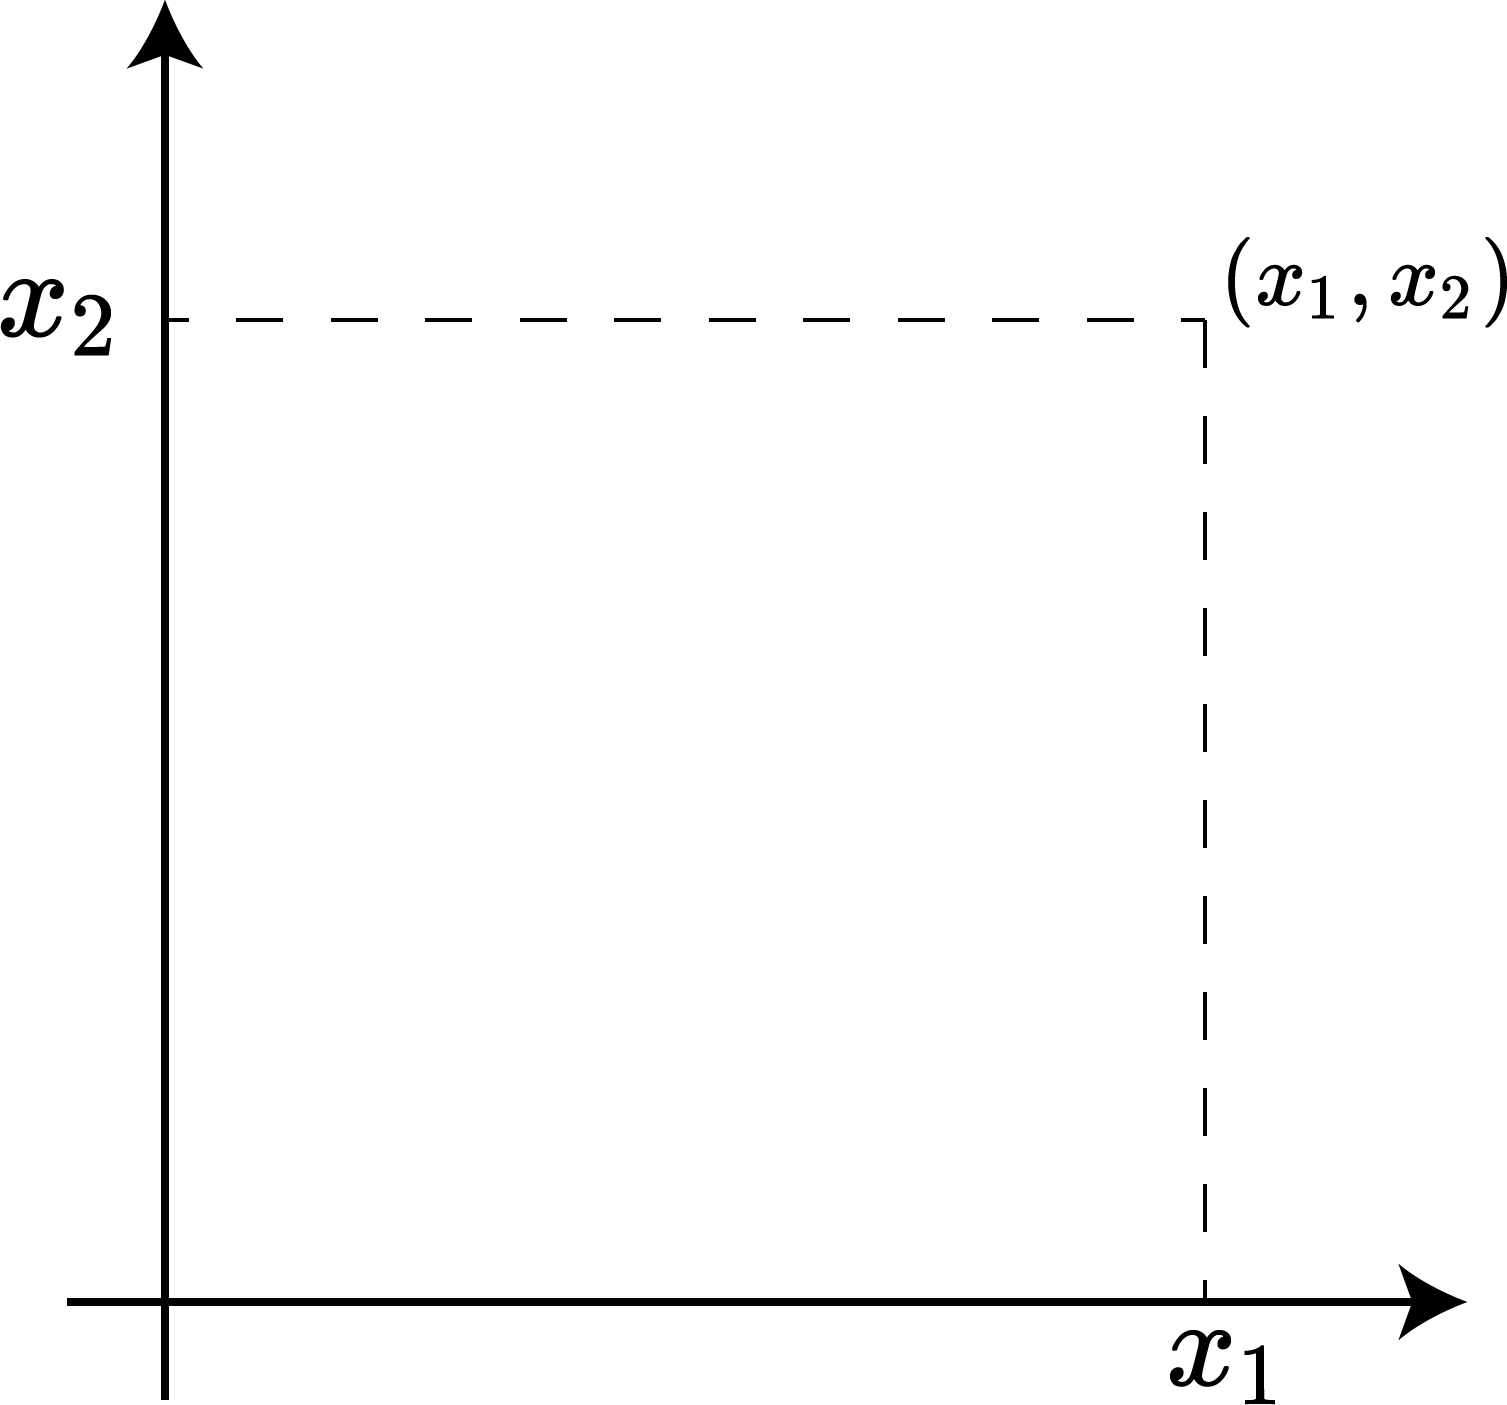
\includegraphics[width=0.3\textwidth]{images/img03.png}\\
\underline{2. Abbildungen} Projektionen\\
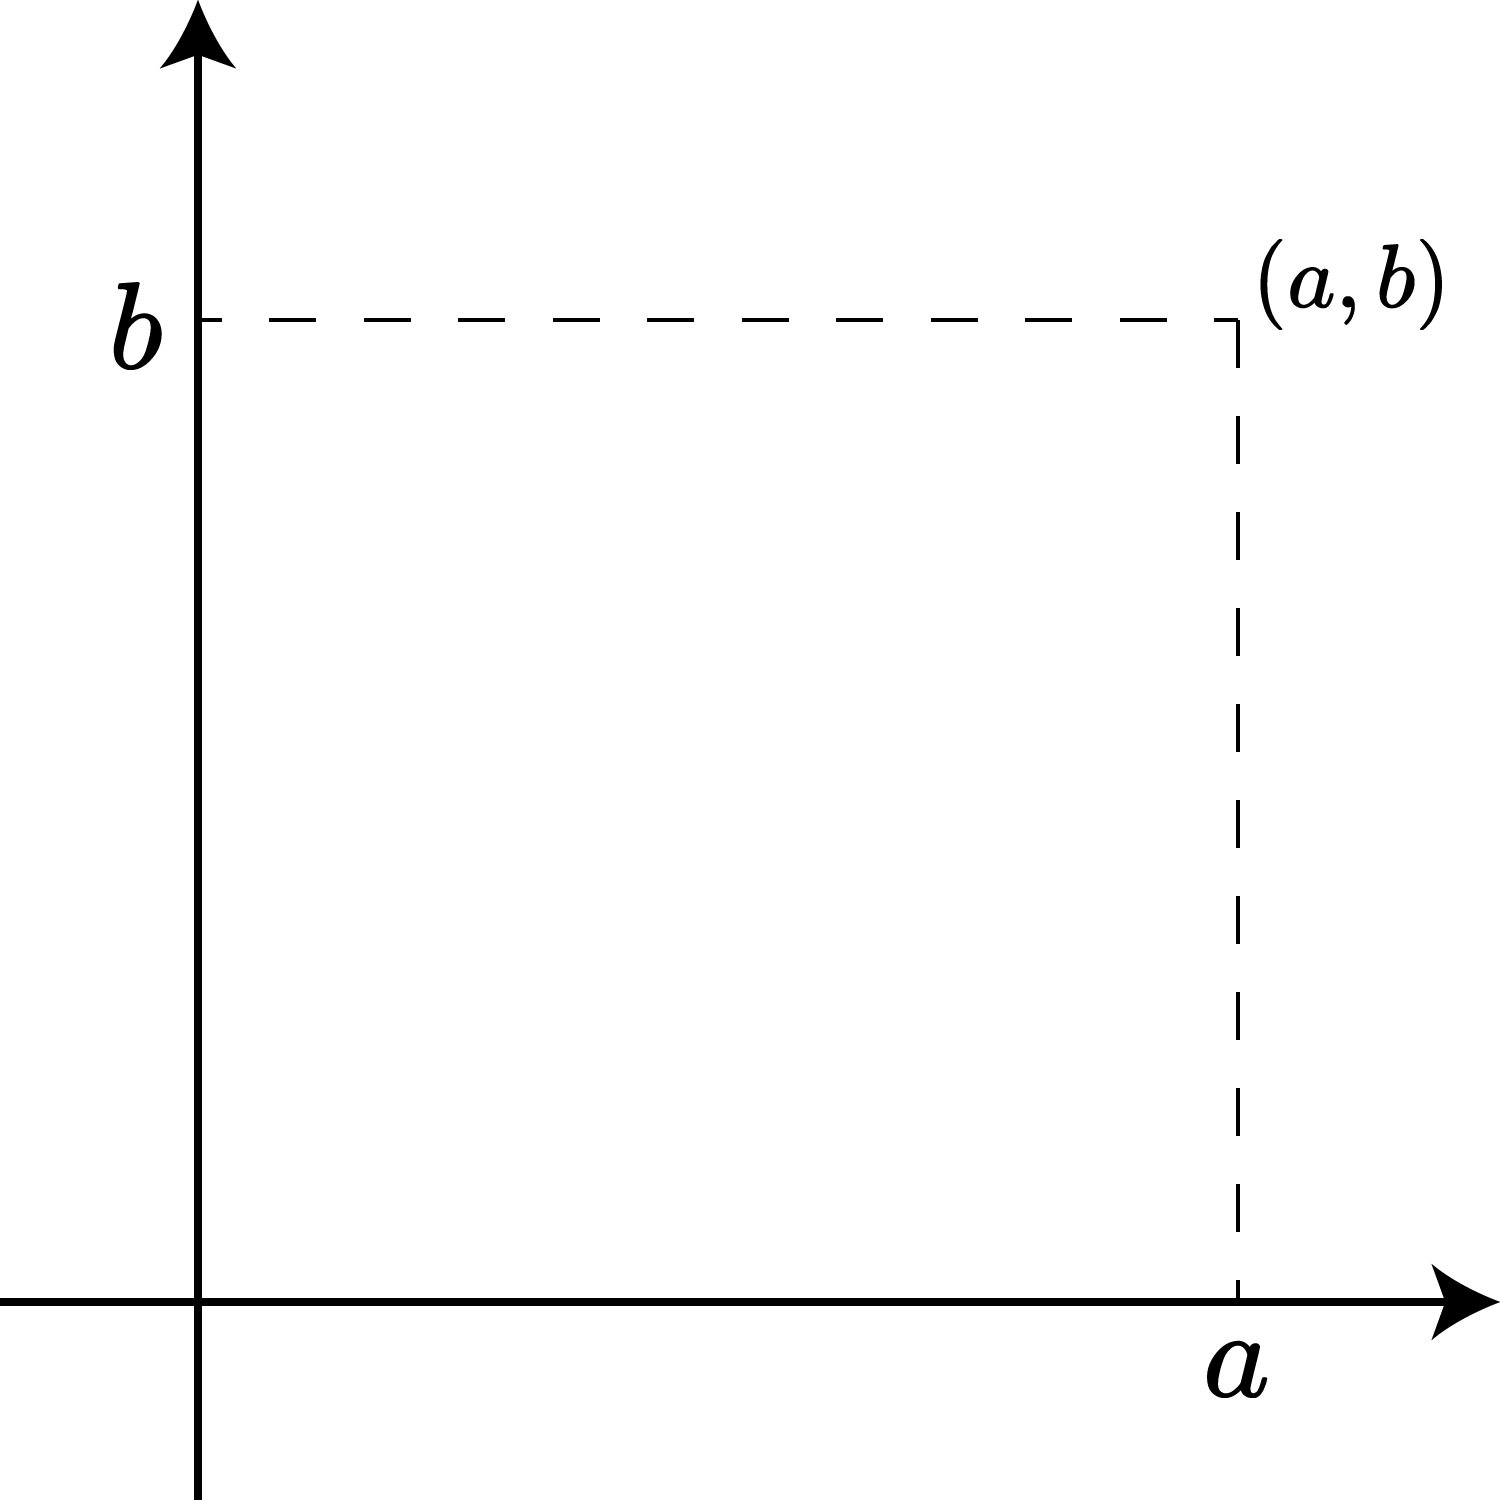
\includegraphics[width=0.3\textwidth]{images/img04.png}\\
$\Pi_1 = \Pi_A : A\times B \rightarrow A, (a,b)\mapsto a$ (Projektion auf 1. Koordinate)\\
$\Pi_2 = \Pi_B : A\times B \rightarrow B, (a,b) \mapsto b$ (Projektion auf 2. Koordinate)\\
$\Pi_A(a,b) = a$\\
$\Pi_B(a,b) = b$\\
$n$-Tupel: Mengen $A_1,\dots ,A_n, n\in \mathbb{N}.$\\
$A_1\times A_2$ wie vorhin\\
$A_1\times\dots\times A_{n+1} := (A_1\times\dots\times A_n)\times A_{n+1}, n\in \mathbb{N}$ (induktiv)\\
\underline{Beobachtung:}\\
$(A\times B)\times C = A\times (B\times C) + \{(a,b,c)|a\in A, b\in B, c\in C\} = ((a,b),c) = (a,(b,c))$\\
Genauer: $\exists$ Bijektion $\Phi : (A\times B) \times C \rightarrow A\times (B\times C)$

\begin{defi}[Graph einer Abbildung]
	Geg: $f: A \rightarrow B$ Funktion\\
	$\Gamma := \Gamma_f := \{(a,b) \in A\times B : b = f(a)\} \subset A\times B$\\
	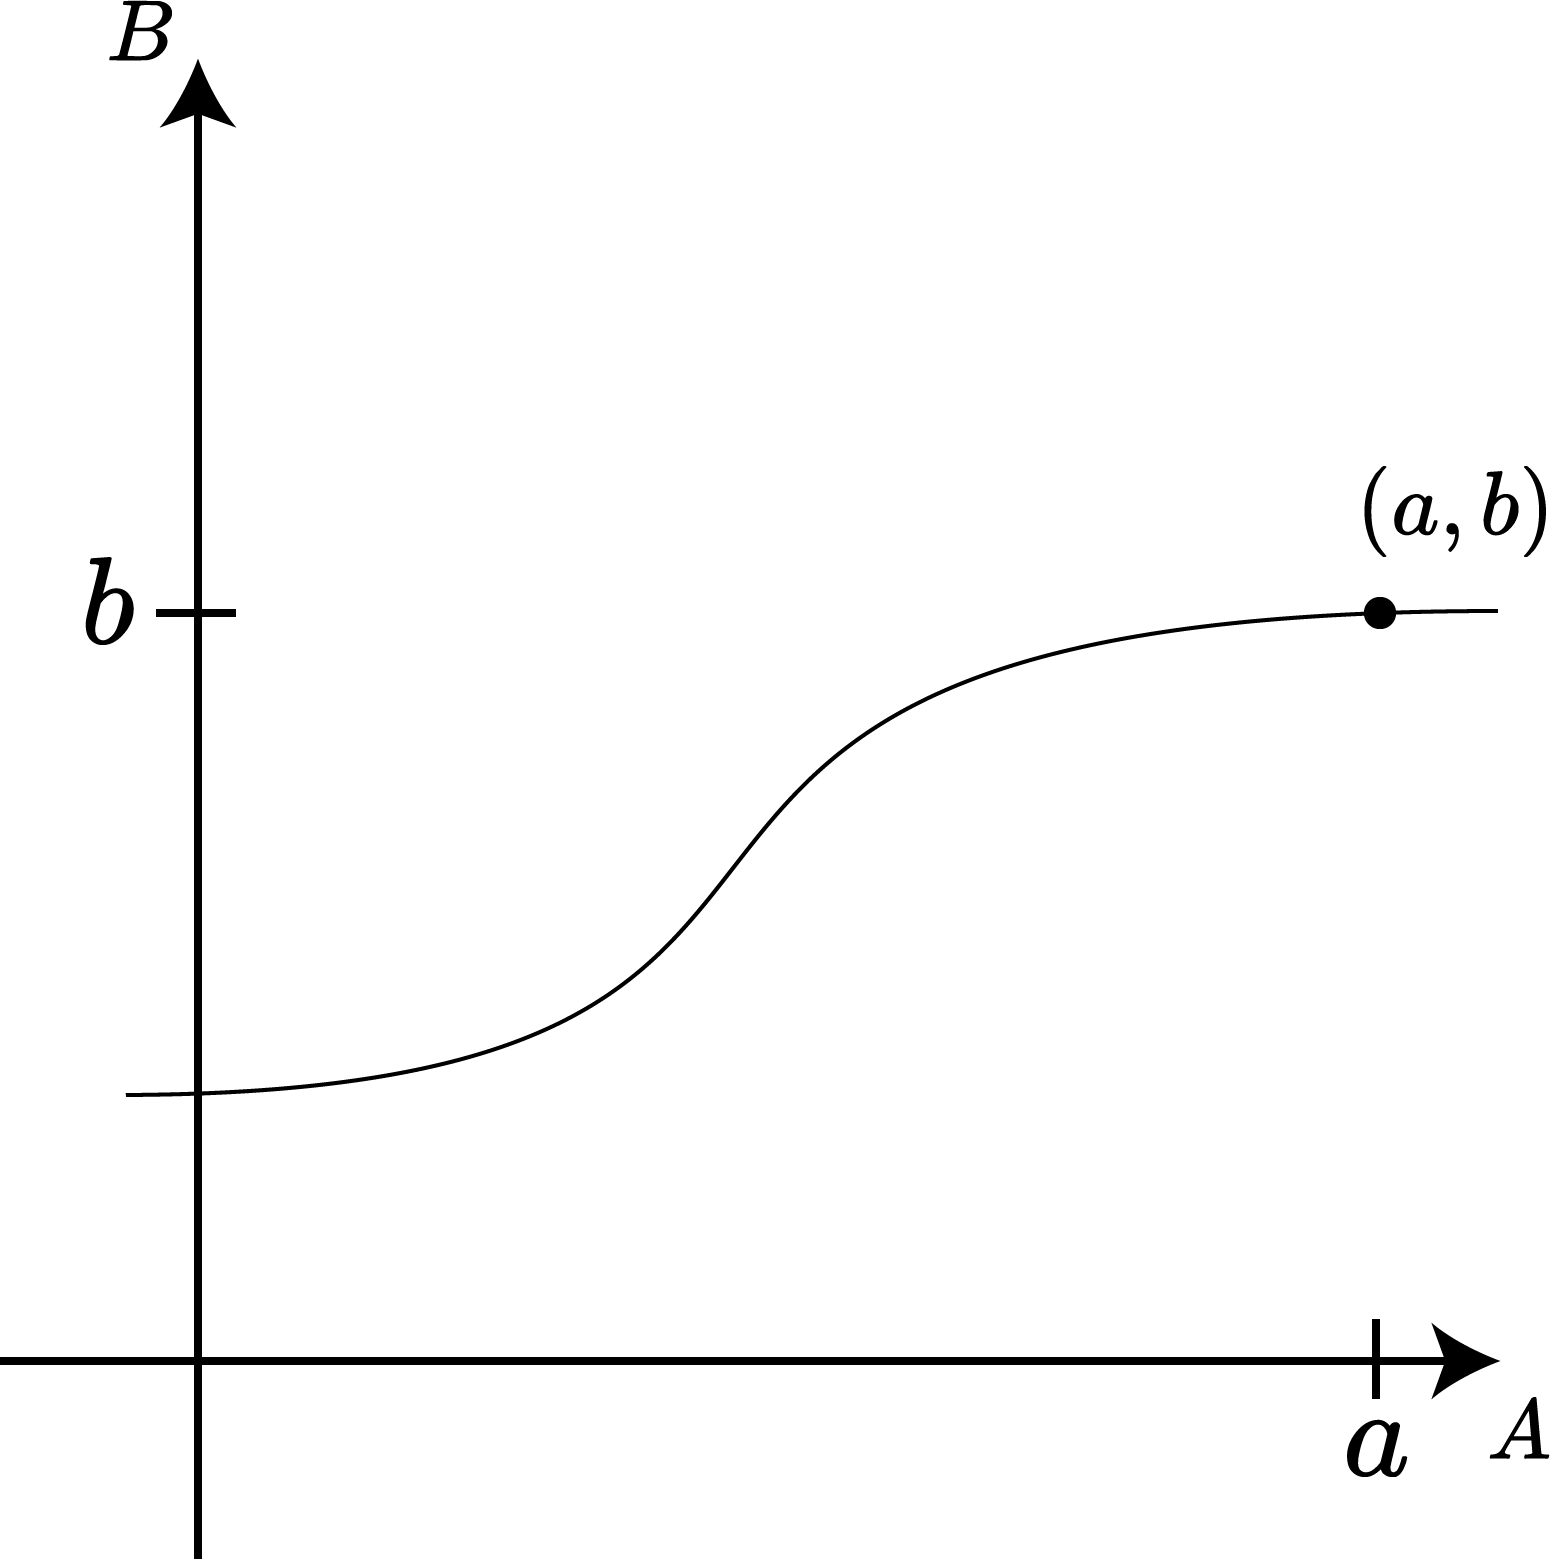
\includegraphics[width=0.3\textwidth]{images/img05.png}
	\quad
	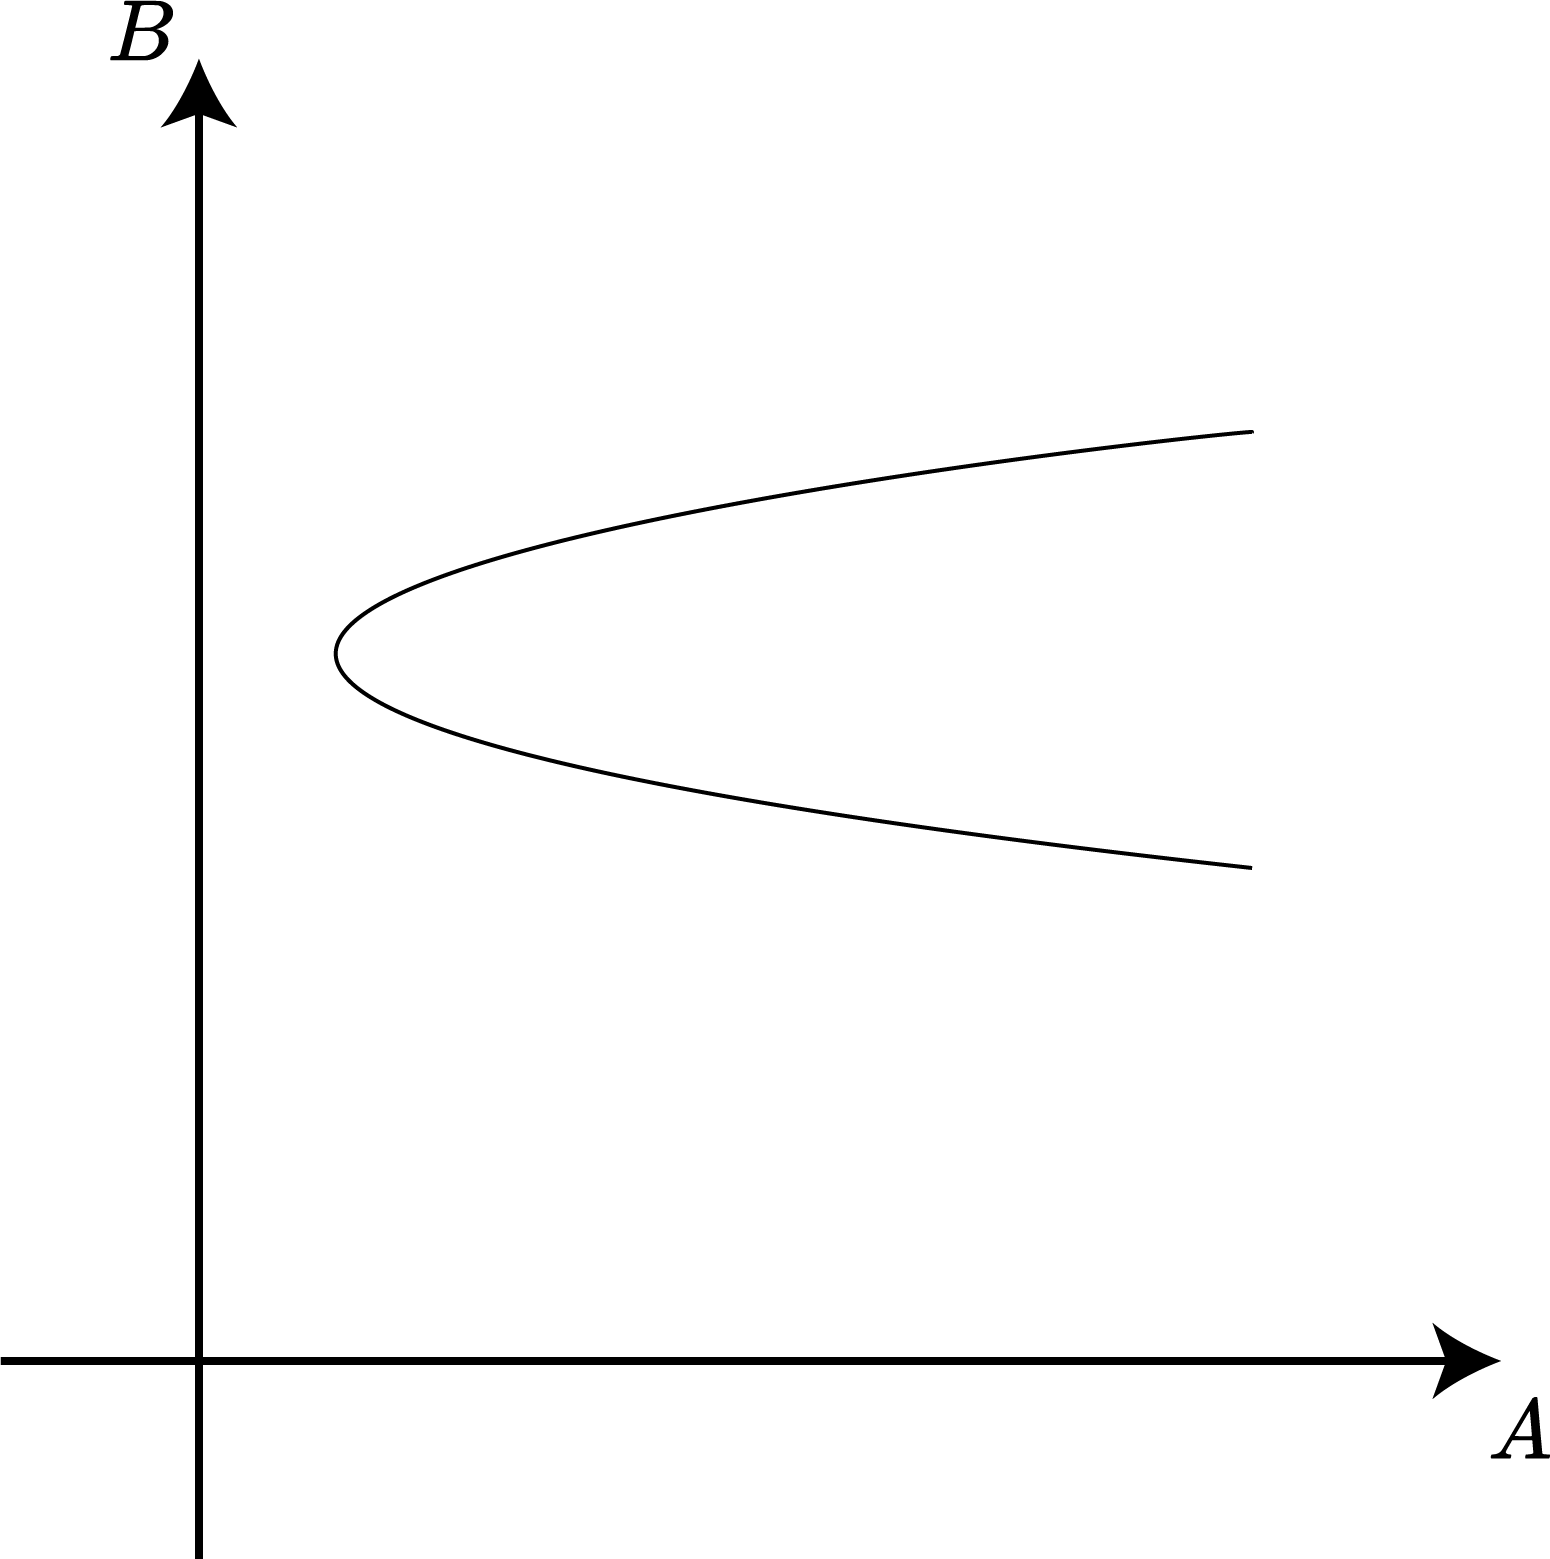
\includegraphics[width=0.3\textwidth]{images/img06.png}\\
	$P\subset A\times B$ ist der Graph einer Funktion genau dann, wenn aus $(a_1,b_1), (a_2,b_2) \in \Gamma$ folgt $b_1 = b_2$. (und $\forall a\in A \exists b\in B:(a,b)\in\Gamma$)
\end{defi}
\begin{satz}
	$\Gamma \subset A\times B$ ist genau dann Graph einer Abbildung $f: A\rightarrow B$, wenn die Projektion $\Pi_A \vert_\Gamma : \Gamma \rightarrow A$ bijektiv ist.\\
	Notation: $g: D \rightarrow E, X\subset D$\\
	$g\vert_X: X\rightarrow E, x\mapsto g(x)$\\
\end{satz}
\begin{bew}
	Sei $\Gamma = \Gamma_f$ mit $f: A\rightarrow B$ Funktion\\
	$\overset{(a,b)\in \Gamma_f \Leftrightarrow b = f(a)}{\Rightarrow} \forall a\in A$ existiert genau ein $b\in B$ mit $f(a) = b$.\\
	$\Rightarrow \Pi_A \vert_\Gamma$ ist bijektiv.\\
	Umgekehrt: Sei $\Pi_A \vert_\Gamma \rightarrow A$ bijektiv.\\
	D.h. ist $(a_j, b_j) \in \Gamma, j \in\{1,2\}$\\
	und $\Pi_A(a_1, b_1) = \Pi_A(a_2, b_2) \Rightarrow (a_1, b_1) = (a_2, b_2)$\\
	$\Leftrightarrow a_1 = a_2, b_1 = b_2$\\
	$\Rightarrow$ zu $a\in A \exists ! b\in B, (a,b) \in \Gamma$.\\
	Da $b=\Pi_B(a,b) = \Pi_B((\Pi_A\vert_\Gamma)^{-1}(a))$\\
	Definiere $f:= \Pi_B \circ (\Pi_A\vert_\Gamma)^{-1}:A\rightarrow B$ ist Funktion\\
	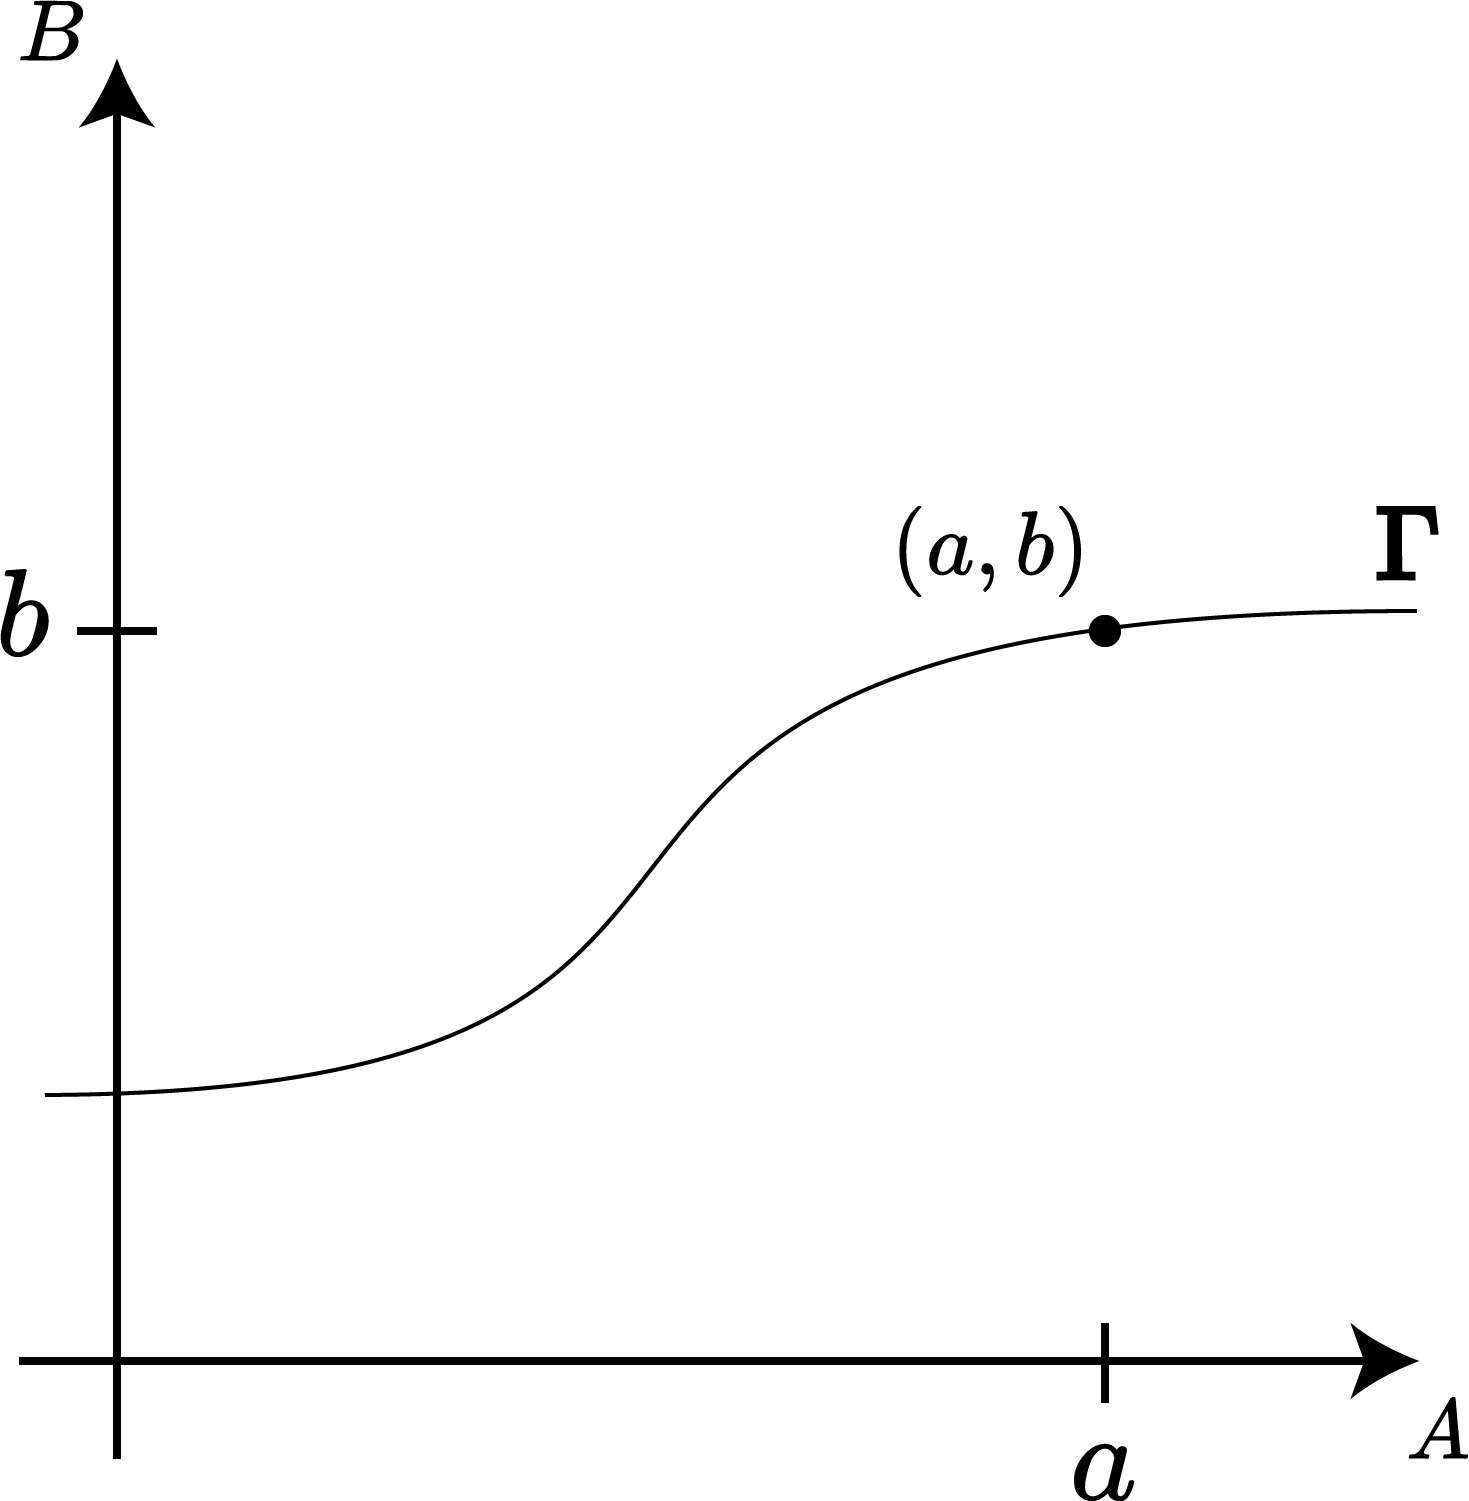
\includegraphics[width=0.3\textwidth]{images/img07.png}\\
	nachrechnen $\Gamma = \Gamma_f$
\end{bew}
\begin{bem}
	In Satz 3 gilt $f = \Pi_B \circ (\Pi_A\vert_\Gamma)^{-1}$ %ENTSPRICHT 4.2
\end{bem}
\begin{bsp}
	Ist $f: A\rightarrow B$ bijektiv\\
	$b=f(a),\quad f^{-1}(b)=a$\\
	Dann gilt: $\Gamma_f^{-1} = \{(b, f^{-1}(b)) | b\in B\}\\
	= \{(f(a),a):a\in A\} = S(\Gamma_f), S: A\times B \rightarrow B\times A$ (swap), $(a,b)\mapsto(b,a)$.\\
	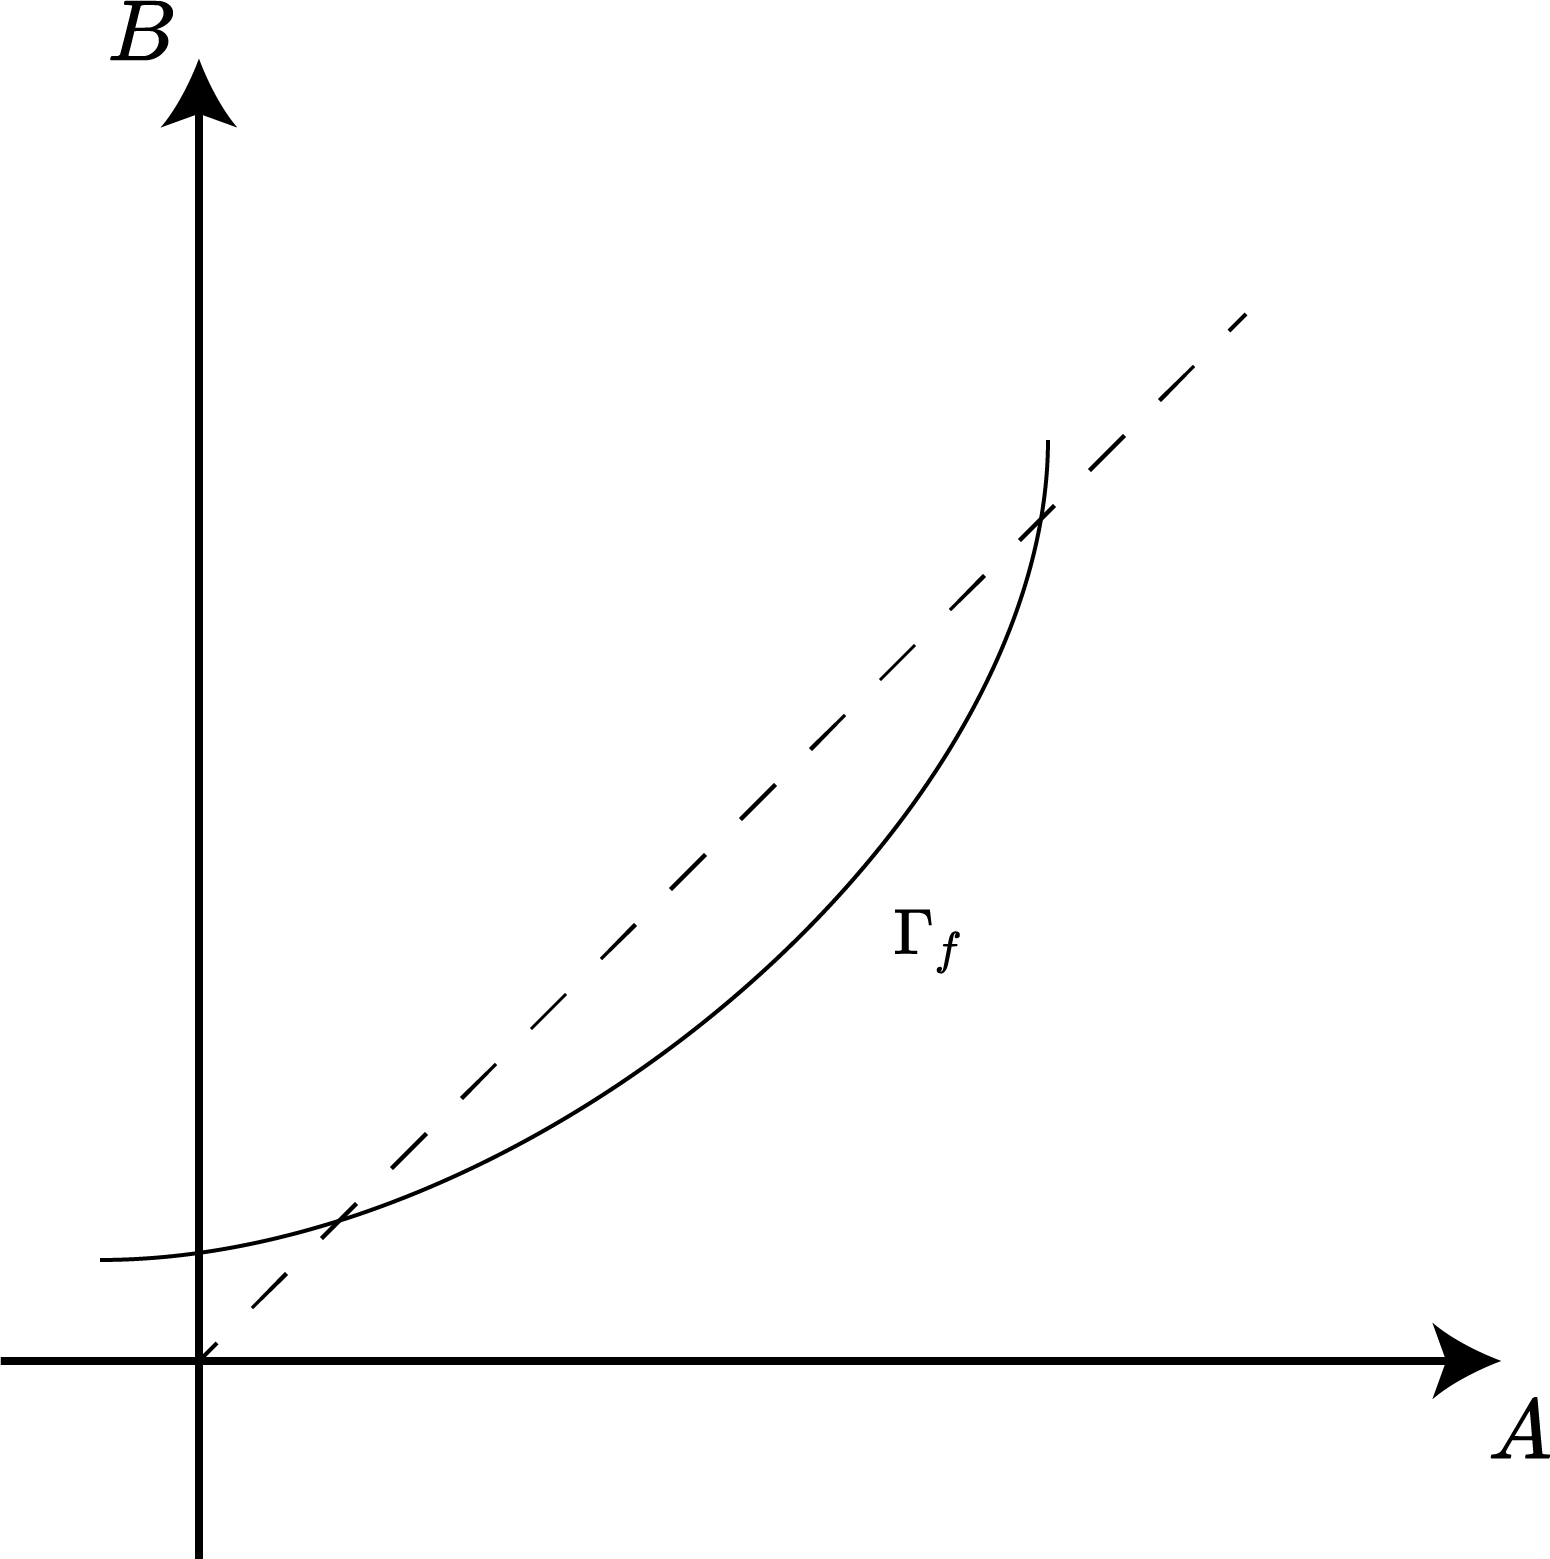
\includegraphics[width=0.3\textwidth]{images/img08.png} \quad
	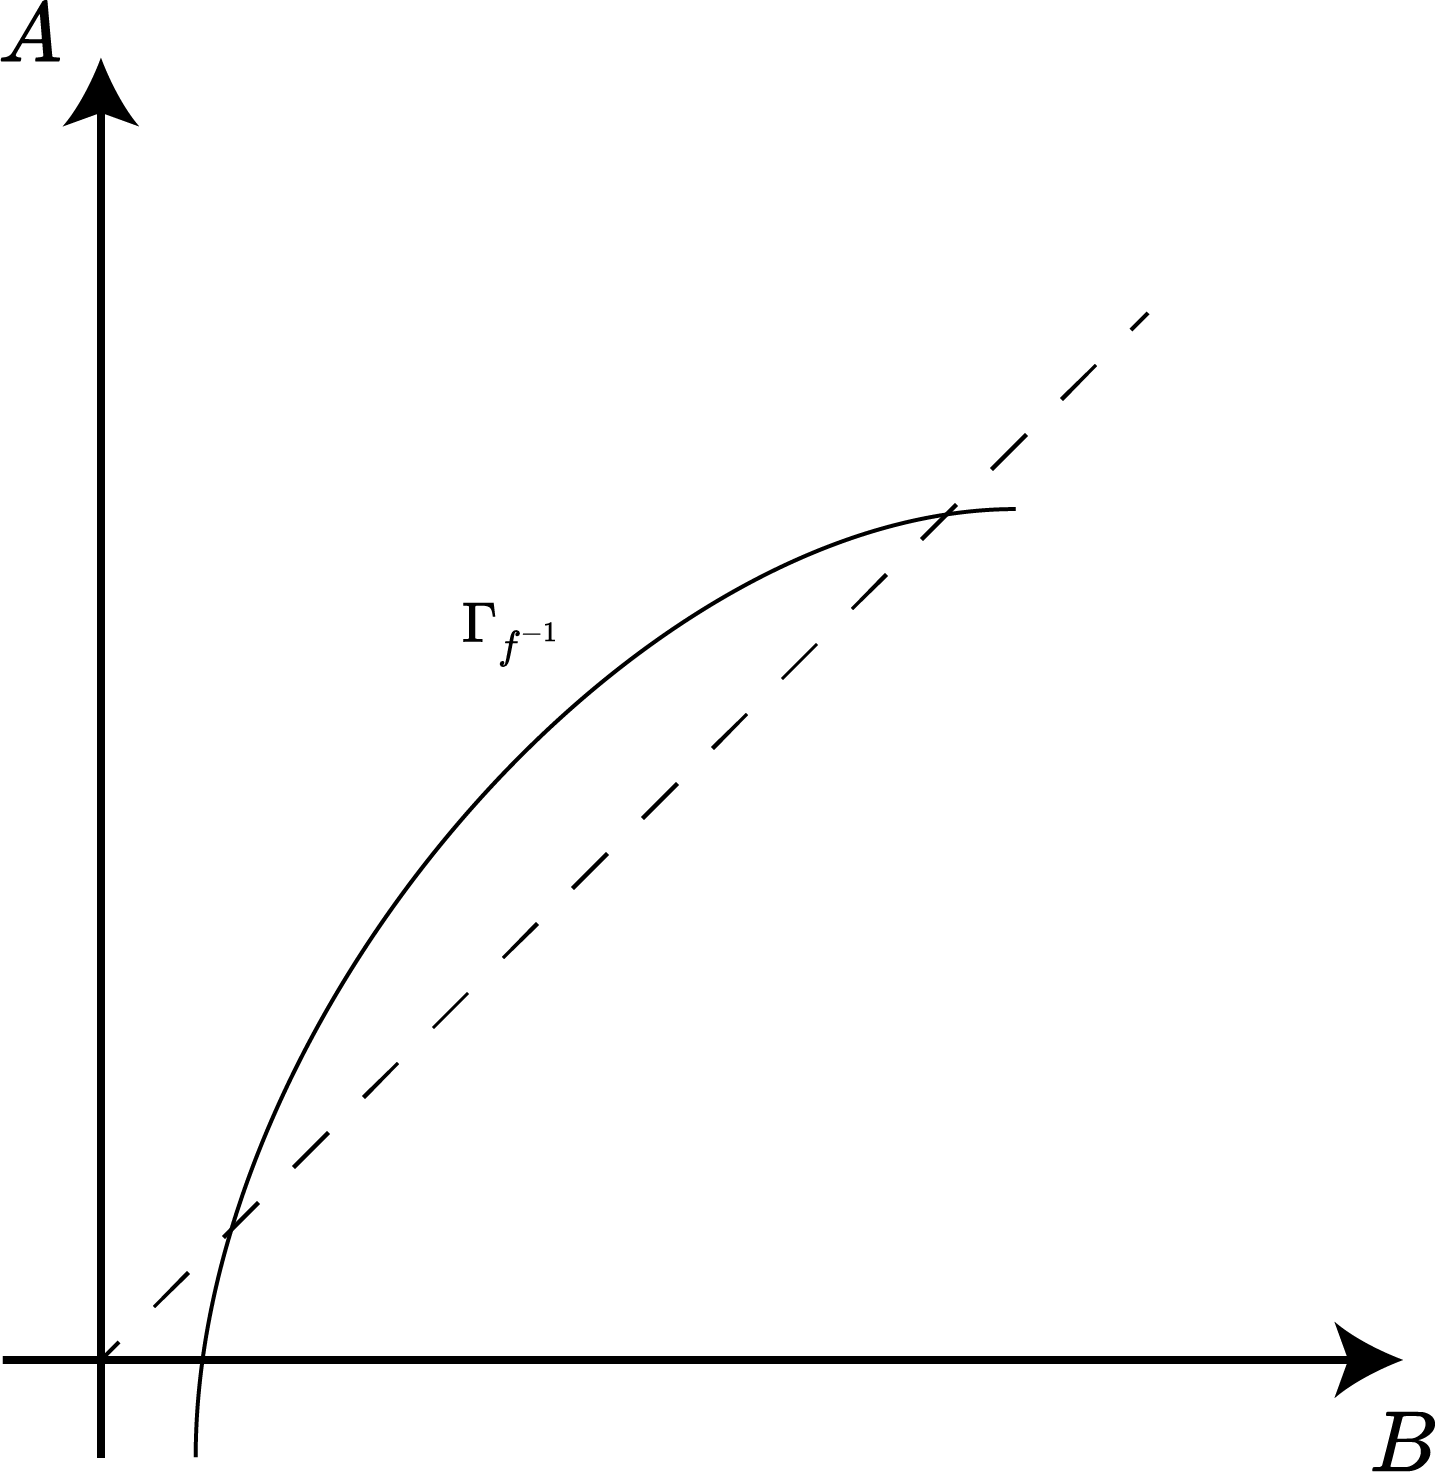
\includegraphics[width=0.3\textwidth]{images/img09.png}\\
	$\Gamma_{f^{-1}} = $ Spiegeln von $\Gamma_f$ an Winkelhalbierenden.
\end{bsp}
\subsection{Schubfachprinzip und endliche Mengen}

\end{document}